\documentclass[12pt, a4paper]{report}
\usepackage[utf8]{inputenc}
\usepackage{float}
\usepackage{csquotes}
\usepackage[german]{babel}
\usepackage{hyperref}
\usepackage[onehalfspacing]{setspace}
\usepackage{geometry}
\usepackage{color}
\usepackage{listings}
\usepackage{graphicx}
\usepackage{acronym}
\usepackage{pgfplots}
%\usepackage{chngcntr}
%\counterwithout{figure}{chapter}
\usepackage{caption}
\DeclareCaptionFormat{citation}{%
   \ifx\captioncitation\relax\relax\else
     \captioncitation\par
   \fi
   #1#2#3\par}
\newcommand*\setcaptioncitation[1]{\def\captioncitation{\textit{Quelle:}~#1}}
\let\captioncitation\relax
\captionsetup{format=citation,justification=centering}
 
\usepackage{amsmath}
\usepackage{amssymb}

%\usepackage[normalem]{ulem}
%\useunder{\uline}{\ul}{}
\usepackage{lstautodedent}
\usepackage{dirtree}

\usepackage[backend=biber,
bibstyle=alphabetic, 
citestyle=authortitle-ibid,
natbib=true, 
hyperref=true,
]{biblatex}
\addbibresource{lit.bib} 
\setcounter{secnumdepth}{3}
\setcounter{tocdepth}{3}
\geometry{
left=2.5cm,
right=2.5cm,
top=2.5cm,
bottom=2.5cm,
bindingoffset=5mm,
}
\definecolor{commentgreen}{RGB}{64, 128, 0}
\definecolor{stringred}{RGB}{179, 0, 0}
\definecolor{codebg}{RGB}{249, 248, 238}
\lstdefinestyle{custompython}{
	language=Python,
	backgroundcolor=\color{codebg},
	breaklines=true,
	commentstyle=\color{commentgreen},
	stringstyle=\color{stringred},
	keywordstyle=\color{blue},
	numbers=left,
	showstringspaces=false
}
\pagestyle{empty}
\begin{document}
%\documentclass[titlepage, 12pt]{scrbook}
%\usepackage[utf8]{inputenc}
%\usepackage[german]{babel}
%\usepackage{uarial}
%\usepackage{color}
%\renewcommand{\familydefault}{\sfdefault}
%\usepackage{fancyhdr}
%\usepackage{graphicx}
%\pagestyle{empty}
%\begin{document}
\begin{titlepage}
	\begin{flushleft}
	\begin{figure}
		\hspace*{-0,5cm}
		
\includegraphics[scale=0.25]{Bilder/DHBW_logo.jpg} \hspace*{5cm}
		
\includegraphics[scale=0.25]{Bilder/Atos_logo.png}
	\end{figure}
	\end{flushleft}
	\vspace*{-0.6cm}
	\begin{center}
	\textcolor{red}{Emotionsanalyse am Beispiel der Pokerfaceerkennung} \par \vspace*{0,5cm}
	Projektarbeit \par \vspace*{2cm}
	des Studienganges \textcolor{red}{Angewandte Informatik / Betriebliches Informationsmanagement}
	an der Dualen Hochschule Baden-Württemberg Mannheim \par \vspace*{1cm}
	von \par \vspace*{0,5cm}
	\textcolor{red}{Fabian Brandmüller, Maximilian Ludwig, Kevin Wrona} \par \vspace*{1cm}
	\today \par \vspace*{2cm}
	\begin{tabular}{l@{\hspace{3cm}}r}
		Bearbeitungszeitraum & \textcolor{red}{23.09.2019 - 24.04.2019} \\
		Betreuer der DHBW & \textcolor{red}{Prof. Dr. Eckhard Kruse} \\[1cm] 
	\end{tabular}
	\end{center}
\end{titlepage}
%\end{document}
\setlength{\parindent}{0em} 
\let\cleardoublepage\relax
\addtocontents{toc}{\protect\thispagestyle{empty}}
\addtocontents{lof}{\protect\thispagestyle{empty}}


\section*{Erklärung}
Ich versichere hiermit, dass ich meine Projektarbeit mit dem Thema: ''Titel der großen Studienarbeit'' selbstständig verfasst und keine nderen als die angegeben Quellen und Hilfsmittel benutzt habe.
\newline
\newline
\newline
\newline
---------------------------------------------       ------------------------------------------ \newline
Ort	\hspace{2cm}		Datum\hspace{3,5 cm}				    Unterschrift
\newpage
\section*{Abstract}
\section*{Abkürzungen}
\begin{acronym}[Bash]
% \acro{VCS}{Version Control System}
\end{acronym}
\newpage
%\renewcommand*{\chapterpagestyle}{empty}
\renewcommand{\thefigure}{\Alph{figure}}
\renewcommand{\thetable}{\Alph{figure}}

\tableofcontents
\listoffigures
\listoftables
\lstlistoflistings
\newpage
\chapter{Einleitung}
\pagestyle{plain}
\setcounter{page}{1}
''Several researchers have stated that facial expression recognition appears to play one of the most important roles in human communication'' 
\footcite[Vgl.][1]{FaceRec}
Dieses Zitat von Katherine B. Leeland gibt einen Einblick in die Relevanz der Emotionserkennung für den Menschen. Fragen zu dieser Thematik stellen sich allerdings nicht erst seit Beginn der Digitalisierung. Bereits Darwin
fragte sich, ob von den Gesichtsausdrücken einer Person nicht auch der Emotionale Zustand abgeleitet werden kann.
\footcite[Vgl.][2]{FaceRec}
Einen solchen Zustand von einem Mitmenschen mittels Software abzulesen ist jedoch nicht nicht leicht zu realisieren. Bereits durch kleine Änderungen in der Mimik werden verschiedene Emotionen ausgedrückt. Zum Beispiel indem eine Person die Lippen zusammen presst und die Augen zusammen kneift bei Wut, oder die Mundwinkel nach unten gezogen werden bei Trauer.
\footcite[Vgl.][249]{HandbookFaceRec}
Durch derartige Ausdrücke können Emotionen wie Wut oder Trauer Ausdruck gewinnen.
Emotionserkennungssoftware gibt es bereits und wird auch in der Wirtschaft eingesetzt. Die Anwendungsgebiete reichen dabei von Jobinterviews, in denen analysiert wird in wie weit die Bewerber für
den jeweiligen Job geeignet sind, 
\footcite[Vgl.][]{mixedArticle}
bis hin zur Automobilindustrie. Dort wird mittels geeigneter Sensorik versucht die Emotion und somit der physiologische Zustand des Autofahrers zu analysieren.
\footcite[Vgl.][Herausforderung]{Frauenhofer}
Diese Daten legen den Grundbaustein für Warnsysteme, welche den Fahrer darauf hinweisen können, dass sein Zustand ungeeignet zum Betrieb eines Kraftfahrzeugs ist. Jedoch werden
solche Einsatzszenarien auch durchaus kontrovers diskutiert. Auf Kritik stößt unter anderem dass die sogenannten ''Basisemotionen'' - z.B. Wut, Trauer, Ekel, Freude, Furcht, Überraschung - , die verwendet werden um den KIs Emotionserkennung
beizubringen, selbst umstritten sind.
\footcite[Vgl.][]{SZ}
Aber auch ethische bedenken werden zunehmend geäußert, vor allem bezüglich der Anwendungsgebiete. Denn je nach Emotion die erkannt werden soll, liegt die Fehlerrate sehr hoch. So hat das
Frauenhofer Institut, welches an Einsatzgebieten von Emotionserkennung in Fahrzeugen arbeitet, festgestellt, dass eine Emotionserkennung je nach Zielemotion eine Vorhersagekraft zwischen 6 und
95\% haben kann.
\footcite[Vgl.][Ergebnis]{Frauenhofer}
Diese negativen Aspekte treffen jedoch nur teilweise auf das hier behandelte Forschungsprojekt zu, wie im Folgenden dargelegt werden soll:
Basierend auf den zuvor genannten Basisemotionen Wut, Frucht, Trauer, Freude, und Ekel soll in dieser Arbeit getestet werden, in wie weit eine technische Vorhersage der Emotionen mittels küünstlicher Intelligenz möglich ist. Dies erfolgt am Anwendungsbeispiel der Pokerface Erkennung. Mittels der hier entworfenen technischen Lösung soll daher getestet werden in wie fern ein Pokerface, das auch als ein emotional neutraler Zustand definiert werden kann, erkannt werden kann.
Diese Forschungsarbeit hat also nicht das Ziel, dass alle oder eine Emotion korrekt vorhergesagt wird, sondern zu ermitteln wann keine Emotion vorliegt.
Das aus dieser Arbeit hervorgehende Prototyp  ist dabei jedoch theoretisch gesehen nicht an das hier verwendete Fallbeispiel des Pokerspielens gebunden. Die Grundidee dieses Prototypen lässt einige hypothetische Einsatzszenarien in der Praxis zu.
 Diese haben eine gewisse Schnittmenge mit denen von ''normaler'' Emotionserkennungssoftware, jedoch gibt es auch einige weitere. Diese  Im Folgenden werden
einige denkbare Szenarien expliziert:
\begin{itemize}
	\item{Polizeiverhöre}
\end{itemize}
Es ist denkbar, dass eine erweiterte Form des entwickelten Prototypen bei Polizeiverhören eingesetzt werden könnte. Hierdurch könnten Beamte die Anwendung eines Pokerfaces durch den Beschuldigten erkennen, welches auf eine Lüge hinweisen könnte. Neben der gebräuchlichen Verwendung eines Lügendetektors wäre der Einsatz der in dieser Arbeit erstellten Lösung eine kostengünstige Variante.
\begin{itemize}
	\item{Gerichtsverhandlungen}
\end{itemize}
Das zweite Einsatzgebiet ist ähnlich zu dem ersten. Bei Gerichtsverhandlungen gelten die gleichen Voraussetzungen wie bei einem Verhör der Polizei. Zwar müssen die Vorgeladenen eine
eidesstattliche Erklärung abgeben nur die Wahrheit zu sagen, jedoch ist zu bezweifeln ob dies auch immer der Fall ist.
Nun soll nicht der Eindruck entstehen dass das hier gebaute Werkzeug ein Lügendetektor ist. Es ist ebenfalls nicht möglich, dass von einem Pokerface immer auf eine Lüge geschlossen werden kann.
Jedoch ist ein Pokerface ein Zeichen dafür, dass sich diese Person ihren emotionalen Zustand nicht anmerken lassen möchte. Und dies wiederum deutet eher daraufhin dass die Person nicht die
Wahrheit sagt oder nur teilweise.
\begin{itemize}
	\item{Pokerspiel}
\end{itemize}
Wie bereits erwähnt ist dieses Einsatzszenario das Fallbeispiel dieser Arbeit. Dies liegt unter anderem daran, dass der erste Begriff der mit dem Wort Pokerface - bzw. einem emotionslosen Gesichtsausdruck -  in Verbindung gebracht wird, das Pokerspiel selber ist. 
Und auch in diesem kann es nützlich sein zu wissen, ob die Kontrahenten ein Pokerface aufsetzen, oder nicht. 
Denkbar wäre es, dass ein Mitspieler zum Beispiel mittels einer Kamera das Gesicht des Gegenübers scannt und analysiert ob ein Pokerface vorliegt oder nicht, und dementsprechend agiert.

\chapter{Anforderungen}
Das nun folgende Kapitel thematisiert die konkrete Aufgabenstellung der Arbeit, so wie eine Anforderungsanalyse mittels MoSCoW Priorisierung. 
\section{Aufgabenstellung}
Das Projekt selber wird an der DHBW in Mannheim durchgeführt und von Prof. Dr. Erckhard Kruse betreut.
Wie eingangs erwähnt soll mittels künstlicher Intelligenz erkannt werden, ob eine Emotion vorliegt oder nicht.
Zur Umsetzung dieser Aufgabe wird eine Bilderkennungssoftware angefertigt, welches ein übermitteltes Bild nach vorhandenen Emotionen analysiert. Sollte keine Emotion durch die Software erkannt werden, wird dem Anwender das Vorhandensein eines Pokerfaces zurück gegeben. Ein konkretes Einsatzgebiet nach Abschluss der Entwicklung ist nicht
vorgesehen, da es sich um ein Forschungsprojekt handelt. Jedoch sind wie bereits in der Einleitung beschrieben einige verschiedene Einsatzmöglichkeiten denkbar, an die das Werkzeug leicht angepasst werden kann.

\section{Usecase}
Wie bereits erwähnt ist der hier behandelte Use Case das Pokerspiel selber. An diesem soll ermittelt werden, in wie weit sich Emotionen vorhersagen lassen können, bzw. das Abhandensein von Emotionen. Dieses Fallbeispiel wurde gewählt, da es unter anderem das naheliegendste ist, so wie ein simples und leicht zu konstruierendes Szenario impliziert. Dabei soll mittels einer Kamera ein Bild von einem Pokerspieler aufgenommen werden, und dann mittels dem hier entworfenen Prototypen verarbeitet und anbalysiert werden. Am Ende soll dann eine Vorhersage der Emotionen getätigt werden die dem Photographen zur Verfügung gestellt wird.


\section{MoSCoW Priorisierung}
Diese Arbeit soll methodisch mit der MoSCoW Priorisierung bearbeitet werden. Diese Art der Priorisierung teilt die zu bearbeitenden Anforderungen in vier Kategorien ein:
\footcite[vgl.][90]{Projektmanagement}
\begin{itemize}
\item Must - Core Anforderungen die unbedingt umgesetzt werden müssen
\item Should - Anforderungen die ebenfalls umgesetzt werden müssen, jedoch um Nachhinein noch durch Change Request verändert werden können.
\item Could - Anforderungen die Nach den Must und Should Anforderungen umgesetzt werden sollen, sofern noch Ressourcen und Zeit vorhanden sind um diese zu bearbeiten
\item Won't - Anforderungen die nicht in diesem Projekt bzw. Release erfolgen, jedoch in einer zukünftigen Version bearbeitet werden sollen. 
\end{itemize}
Im Zuge des Projektes wurden die vorhandenen Anforderungen wie folgt anhand der MoSCoW Priorisierung eingeordnet:
\begin{itemize}
\item Must
\begin{itemize}
\item Emotionen werden nicht zufällig erkannt
\item Es wird zwischen keine Emotion (Pokerface) und Emotion vorhanden unterschieden
\item Benutzerfreundliche Interaktionsmöglichkeit um Input zu liefern und Output darzustellen
\end{itemize}
\item Should
\begin{itemize}
\item Die Wahrscheinlichkeit zur Erkennung der richtigen Emotion muss über 50\% liegen
\item Es können mindestens fünf verschiedene Emotionen erkannt werden
\item Die Erkennung der Emotion darf nicht länger als 30 Sekunden dauern
\item Die Kosten zur Umsetzung der Lösung müssen dem Nutzen gerecht werden?
\end{itemize}
\item Could
\begin{itemize}
\item Bilder können zu Echtzeit analysiert werden
\item Das Trainieren des Modells darf nicht länger als 72 Stunden dauern
\item Eine Oberfläche zur intuitiven Bedienung der Lösung ohne technisches Verständnis muss vorhanden sein
\end{itemize}
\item Won't
\begin{itemize}
\item Neben dem Analysieren von Bildern ist auch die Analyse von Videos möglich
\end{itemize}
\end{itemize}
Dabei sollen die einzelnen Anforderungen entsprechend ihrer Priorität abgearbeitet werden. So kann am Ende der Erfolg der Arbeit deutlich besser eingeordnet werden

\let\cleardoublepage\relax

\chapter{Stand der Technik}
In diesem Abschnitt soll der aktuelle Forschungs- und Entwicklungsstand im Bereich Emotionserkennung thematisiert werden. Jedoch muss dafür erst einmal eine Unterscheidung der Begrifflichkeiten
Emotionserkennung und Gesichtserkennung erfolgen, da beide gebiete Überschneidungen haben, jedoch inhaltlich und von ihren Zielen verschieden sind.

\section{Gesichtserkennung vs. Emotionserkennung}

\subsection{Gesichtserkennung}
Gesichtserkennung ist eine Disziplin der Informatik in der es darum geht Gesichter wieder zu erkennen, und gegebenenfalls verschiedenen Personen zuzuordnen. Dabei lässt sich der Prozess der
Gesichtserkennung in vier Phasen einteilen, Face ''detection'', ''alignment'', ''feature extraction'' und ''matching'', wie anhand von Grafik \ref{fig:Face Recognition} sichtbar ist.
\footcite[Vgl. ][2]{HandbookFaceRec}
\begin{figure}[h]
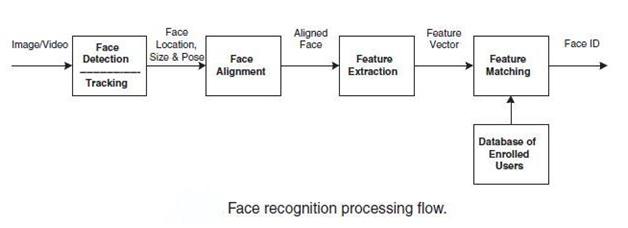
\includegraphics[width=\linewidth]{Bilder/FaceRecognition.png}
\setcaptioncitation{ https://alitarhini.files.wordpress.com/2010/12/untitled1.png}
\caption{ Phasen der Gesichtserkennung}
\label{fig:Face Recognition}
\end{figure}
Die Detection Phase ist dafür verantwortlich um zu erkennen ob Gesichter vorhanden sind in einem Bild, oder aber Video.
\footcite[Vgl. ][2]{HandbookFaceRec}
In der darauffolgenden Alignment Phase hingegen wird die Lokalisierung der Gesichter genauer, indem Gesichtskomponenten wie Augen, Augenbrauen, oder die Nase genauer lokalisiert werden. Dabei
wird das Bild oder Video ebenfalls normalisiert, indem z.B. die Bildbeleuchtung angepasst wird.
\footcite[Vgl. ][2]{HandbookFaceRec}
In der Feature extraction hingegen werden die verschiedenen Gesichtskomponenten wie Augen, Nase, Mund, dem Bild oder Video entnommen. Dies ist ein wichtiger Schritt für weitere Prozesse wie
Eye Tracking oder Face Tracking. Alternativ kann sogar eine bestimmte Person anhand der extrahierten Merkmale erkannt werden.
\footcite[Vgl. ][Abstract]{IEEE}
In der letzten Phase, dem Matching, geht es darum die gewonnen Daten mit den in der Datenbank vorhandenen Gesichtern abzugleichen. Wenn eine genügende Übereinstimmung gefunden wurde, wird ein
Match mit einer Person ausgegeben.
\footcite[Vgl. ][3]{HandbookFaceRec}
Die Anwendungsgebiete von Software die Gesichtserkennung ermöglicht ist mannigfaltig. Sie reicht von Applikationen die ein Gerät wie ein Smartphone entsperren, wenn das Gesicht des Besitzers als
Match ausgegeben wurde, bis hin zur Anwendung in Verbrechensbekämpfung. In jedem dieser Szenarien wird dabei der oben beschriebene Ablauf durchgegangen, und abhängig vom zu liefernden Ergebnis
eine Abschlussaktion vorgenommen.

\subsection{Emotionserkennung}
In diesem Unterkapitel nun sollen Emotionen an sich thematisiert werden, da diese maßgeblich sind für das zu entwickelnde Tool. Eine Definition von Emotionserkennung ist per se nicht schwer zu geben. Prinzipiell beschäftigt sich Emotionserkennung mit der Analyse von Gesichtern und den Emotionen die diese Gesichter darstellen. Jedoch ist der Begriff der Emotionen nicht ganz so einfach zu definieren, wie im folgenden erläutert wird: 

%\begin{itemize}
%\item was ist Emotionserkennu
%\item usecase für emotion recognition
%\item Aiusblick und Kontroverse
%\end{itemize}

\subsubsection{Emotionen}

\begin{itemize}
\item Def. von Emotionen
\end{itemize}
 Grundsätzlich gibt es  verschieden Ansätze Emotionen zu
definieren und einzuteilen. Eine Variante ist dabei die eingangs erwähnte, nicht ganz unumstrittene Einteilung in Basisemotionen. Eine gängige Einteilung ist dabei die verschiedenen
Emotionen in acht Bereiche einzuteilen. Diese Einteilung wurden 1984 von Plutchik postuliert und beinhaltet die Emotionskategorien Angst, Wut, Freude, Trauer, Akzeptanz, Ekel, Erwartung und
Überraschung.
\footcite[Vgl. ][3]{FaceRec}
Jedoch ist dies nicht die einzige mögliche Einteilung. Als weiteres Beispiel teilte MacLean die Emotionen in lediglich sechs Kategorien ein, welche da wären: Verlangen, Wut, Angst,
Niedergeschlagenheit, Freude und Zuneigung.
\footcite[Vgl. ][3]{FaceRec}
Wie sich bereits an den beiden Beispielen zeigt, geht die Meinungen der Forscher dabei  stark auseinander, welche und wie viele Emotionen zu den sogenannten ''Basis Emotionen'' gehören. In
dieser Arbeit werden die Emotionen in sechs Kategorien eingeteilt, in Wut, Trauer, Freude, Ekel, Überraschung und Neutral. Diese Einteilung entspricht an sich keiner gängigen Einteilung, jedoch
wurde diese aus den folgenden Gründen gewählt: \newline
Die hier genannten Emotionen lassen sich gut anhand von Bildern erlernen, da diese zum Teil komplementär und somit eindeutig sind. Es ist aber auch einfacher Testdatensätze zu bekommen für ein
freudiges Gesicht, oder ein überraschtes, als ein Gesicht mit dem emotionalen Ausdruck Akzeptanz. Des Weiteren wurde der Ausdruck ''Neutral'' hinzugefügt. Neutral repräsentiert ein emotionsloses
Gesicht, und somit nach Definition einem Pokerface. Zudem sind die gewählten Emotionen häufig bei dem Test Usecase dieser Arbeit anzutreffen, dem Texas Holdem Poker.

\subsubsection{Abgrenzung zur Gesichtserkennung}
Der grundlegende Unterschied zwischen Emotions- und Gesichtserkennung liegt nun darin, dass bei der Emotionserkennung selber nicht die agierende Person im Vordergrund steht, sondern die Aktion die sie ausführt.
Bei der Gesichtserkennung hingegen spielt lediglich die Rolle wer eine Aktion ausführt, und ob es einen Treffer in der Datenbank gibt, oder nicht. Wegen dieser Unterschiede ist auch die technische Realisierung eines Prototypen, vor allem im Bezug auf die Architektur,  durchaus unterschiedlich. Dies ist jedoch ebenso von den unterschiedlichen Anwendungsszenarien der beiden Verfahren bedingt.
 Denn diese sind ebenso verschieden. Während Gesichtserkennung eher in den Bereich IT-Security oder aber Social Media (Snapchat Filter) eingesetzt wird, ist Emotionserkennung eher Informationsgenerierend.
Zum Beispiel kann durch Emotionserkennung Informationen zugänglich werden wie das Befinden eines Individuums ist, ob emotional betroffen ist, oder aber nicht emotional betroffen wirken möchte und ein Pokerface aufsetzt.
Wegen dieser signifikanten Unterschiede kann daher trotz der Gemeinsamkeiten nicht gesagt werden, dass Emotionserkennung eine Unterkategorie von Gesichtserkennung ist.

\subsubsection{Wann ist ein Gesicht ein Pokerface?}
\label{pokerface}
Bis zu diesem Teil der Arbeit wurden schon immer wieder das Wort Pokerfaces verwendet ohne es formal zu definieren. Jedoch ist es für die Arbeit wichtig eine konkrete Definition für diesen Begriff zu geben, da ansonsten die Anforderungen an die Arbeit nicht korrekt bewertet werden könnten. Da es mehrere Ansätze gibt ein Pokerface zu definieren, wird dies in diesem Abschnitt nachgeholt. Zum einem gibt es den trivialen Ansatz, der bereits am Ende des letzten Kapitels verwendet wurde. Dieser ist, dass ein Pokerface dann vorliegt, wenn ein Subjekt keinerlei Emotion in seinem Gesicht zu erkennen gibt. Dies würde wie bereits erwähnt einer neutralen Emotion entsprechen. Dieser Fall kann auch vergleichsweise einfach behandelt werden, da diese neutrale Emotion auch in die Basisemotionen mit aufgenommen wurde in dieser Arbeit. Das bedeutet, dass beispielsweise ein neuronales Netz auch diese Arten von Gesichtern klassifizieren könnte. \newline
Der zweite Ansatz ist weniger intuitiv, jedoch ebenso wichtig. Es kann durchaus angenommen werden, dass z.B. ein sehr erfahrener Pokerspieler weiß, dass man ein Pokerface einfach identifizieren kann, und demnach alleine dadurch Informationen gewinnen kann. Um dem entgegenzuwirken könnte ein solcher Spieler eine andere Art Pokerface verwenden. Es wäre denkbar, dass ein Spieler versucht sein Gesichtsausdruck permanent gleich zu halten, indem er eben dauerhaft lacht oder lächelt, dauerhaft betrübt, wütend, ängstlich, etc. aussieht. Dieser Ansatz ist weniger intuitiv als der erste und könnte demnach auch weniger schnell erkannt werden.
Mit diesen beiden Definitionen für ein Pokerface wird im Verlaufe der Arbeit gearbeitet.

\section{Emotionserkennung mithilfe von Deep Learning}
In dem nun folgenden Kapitel wird erörtert wie das Ziel des Prototypen dieser Arbeit - das Erkennen eines Pokerfaces - mittels eines neuronalen Netzes umgesetzte werden kann. Dabei wird weniger auf die generellen Eigenschaften von Neuronalen Netzen Bezug genommen, als auf die in dieser Arbeit spezifischen Aspekte. Diese sind vor allem verschieden Ansätze und Möglichkeiten mittels Machine Learning eine Emotionserkennungssoftware zu erstellen.

\subsection{Machine Learning - Frameworks}
Um die gegebene Aufgabenstellung der Erkennung von Emotionen mittels der Analyse eines Gesichtes umsetzen zu können, musste ein entsprechendes Framework Anwendung finden, welches den Anforderungen gerecht wird. Maschinelles Lernen gehört in der heutigen Softwareentwicklung zu den beliebtesten Themen, wodurch dieses schnelle regelmäßige Änderungen und Weiterentwicklungen erfährt. Dementsprechend werden auf dem Markt auch zahllose kostenlose wie auch kostenpflichtige Frameworks angeboten. Um nur einige bekannte aufzuzählen fallen darunter OpenCV, TensorFlow oder Pandas. Möchte man nun das geeignete Framework für das eigene Projekt ausfindig machen, muss man das gegebene Angebot nach einigen Kriterien filtern. Als erstes stellt sich die Frage, was für eine Art von Applikation man umsetzen möchte. Soll das Projekt Texte analysieren oder wie im Falle dieses Projektes die Emotionen aus einem gegebenen Bild? Welche Programmiersprache wird innerhalb des Projektes eingesetzt? Zudem sind Informationen zur Lizenz und dem Support wichtig, sowie insbesondere die Community. 
\newline
Nach entsprechender erster Selektion musste sich schlussendlich zwischen Dlib und Keras entschieden werden, welche für die Umsetzung der Anforderungen dieses Projektes am besten geeignet schienen. Beide Frameworks werden in den folgenden beiden Unterkapitel dem Leser kurz vorgestellt und anschließend wird ein Fazit gezogen, welches der beiden für dieses Projekt am geeignetsten war.

\subsubsection{Dlib}
Dlib ist nach dessen Entwickler Davis King ein modernes C++ Toolkit, welches Machine-Learning Algorithmen und Tools zur Entwicklung komplexer Software enthält um Probleme aus der echten Welt lösen zu können.\footcite[Vgl.]{netguru}
\newline
Dlib selbst wurde in der Programmiersprache C++ entwickelt und kann durch eine Anbindung auch für Python Projekte eingesetzt werden. Die Software-Bibliothek kann unter den Bedingungen der Boost-Lizenz frei genutzt werden und ist durch entsprechende APIs des jeweiligen Betriebssystems Plattformunabhängig. Ein weiterer Vorteil bietet die Unabhängigkeit der Bibliothek von anderen Bibliotheken. %Von Wikipedia (Vlt. andere Quelle suchen)
Dlib ist seit dem Jahr 2002 in Entwicklung und bietet dementsprechend unzählige Features an, welche für verschiedenste Einsatzgebiete verwendet werden können, wie numerische und graphische Modell-Algorithmen und vor allem Gesichtserkennung.\footcite[Vgl.][]{netguru}
Eines der größten Vorteile dieser Bibliothek besteht in der ausführlichen Dokumentation für sämtliche Klassen und Funktionen, wie es nicht häufig der Fall ist für vergleichbare Open-Source Projekte.\footcite[Vgl.]{Dlib}

\subsubsection{Keras}
Die Open-Source Bibliothek Keras wurde im Vergleich zu Dlib im Jahre 2015 von dem Google-Programmierer François Chollet in der Programmiersprache Python entwickelt.\footcite[Vgl.]{Keras}
Bei der Entwicklung von Keras stand die Benutzerfreundlichkeit als eines der wichtigsten Prinzipien im Mittelpunkt. Dem gefolgt bietet Keras eine schnelle und leichte Erstellung neuronaler Netze. Durch ein ausführliches Feedback können Fehler durch den Benutzer schnell ausfindig gemacht und behoben werden. Ein weiteres Designprinzip von Keras ist die Modularität, mithilfe derer man verschiedene Module beliebig konfigurieren und miteinander kombinieren kann. Zudem bietet die Open-Source Bibliothek die Unterstützung von rekurrenten und konvolutionalen Netzwerken, sowie die Unterstützung der GPUs und CPUs, welches für die Umsetzung dieses Projektes von Vorteil waren.
\footcite[Vgl.]{Keras2}
Zuletzt steht hinter Keras eine große aktive Community, welche zahlreiche Tutorials und Hilfestellungen für verschiedenste Problemstellungen liefert.


\subsubsection{Unterschiede}


%\begin{table}[]
%\begin{tabular}{llllllllllllllllll}
%\multicolumn{1}{c}{{\ul \textbf{Software}}} &
%  \multicolumn{1}{c}{{\ul \textbf{Creator}}} &
%  \multicolumn{1}{c}{\textbf{\begin{tabular}[c]{@{}c@{}}Initial \\ Release\end{tabular}}} &
%  \multicolumn{1}{c}{\textbf{\begin{tabular}[c]{@{}c@{}}Software \\ Licence\end{tabular}}} &
%  \multicolumn{1}{c}{{\ul \textbf{Open Source}}} &
%  \multicolumn{1}{c}{{\ul \textbf{Platform}}} &
%  \multicolumn{1}{c}{{\ul \textbf{Written in}}} &
%  \multicolumn{1}{c}{{\ul \textbf{Interface}}} &
%  \multicolumn{1}{c}{{\ul \textbf{OpenMP support}}} &
%  \multicolumn{1}{c}{{\ul \textbf{OpenCL support}}} &
%  \multicolumn{1}{c}{\textbf{\begin{tabular}[c]{@{}c@{}}CUDA\\ support\end{tabular}}} &
%  \multicolumn{1}{c}{\textbf{\begin{tabular}[c]{@{}c@{}}Automatic\\ differentiation\end{tabular}}} &
%  \multicolumn{1}{c}{\textbf{\begin{tabular}[c]{@{}c@{}}Has pretrained\\ models\end{tabular}}} &
%  \multicolumn{1}{c}{\textbf{\begin{tabular}[c]{@{}c@{}}Recurrent\\ nets\end{tabular}}} &
%  \multicolumn{1}{c}{\textbf{\begin{tabular}[c]{@{}c@{}}Convolutional \\ nets\end{tabular}}} &
%  \multicolumn{1}{c}{{\ul \textbf{RBM/DBNs}}} &
%  \multicolumn{1}{c}{\textbf{\begin{tabular}[c]{@{}c@{}}Parallel execution \\ (multi node)\end{tabular}}} &
%  \multicolumn{1}{c}{\textbf{\begin{tabular}[c]{@{}c@{}}Actively\\ Developed\end{tabular}}} \\
%Keras &
%  Francois Chollet &
%  2015 &
%  MIT license &
%  Yes &
%  \begin{tabular}[c]{@{}l@{}}Linux, macOS,\\ Windows\end{tabular} &
%  Python &
%  Python, R &
%  \begin{tabular}[c]{@{}l@{}}Only if using \\ Theano as backend\end{tabular} &
%  \begin{tabular}[c]{@{}l@{}}Can use Theano,\\ Tensorflow or \\ PlaidML as backends\end{tabular} &
%  Yes &
%  Yes &
%  Yes &
%  Yes &
%  Yes &
%  No &
%  Yes &
%  Yes \\
%Dlib &
%  Davis King &
%  2002 &
%  Boost Software License &
%  Yes &
%  Cross-Platform &
%  C++ &
%  C++ &
%  Yes &
%  No &
%  Yes &
%  Yes &
%  Yes &
%  No &
%  Yes &
%  Yes &
%  Yes &
%  
%\end{tabular}
%\end{table}
Zusammenfassen kann gesagt werden, dass Dlib eine mächtige Bibliothek für die Umsetzung verschiedenster Aufgaben ist. Die ausführliche Dokumentation bietet eine große Hilfestellung. Jedoch folgt aus dem Angebot der zahlreichen Features auch eine längere Einarbeitung, bis die Anforderungen produktiv umgesetzt werden können. 
\newline
Keras hingegen bietet durch dessen benutzerfreundliche Entwicklung und den zahlreichen Tutorials eine schnelle erste Umsetzung der Aufgaben. Durch die Modularität und der aktiven Community können viele öffentliche Lösungen genutzt und für die eigenen Anforderungen abgeändert werden. 
Aus diesem Grund und aufgrund der Unterstützung der rekurrenten und konvolutionalen Netzwerken wurde sich für die Verwendung von Keras als Open-Source Bibliothek in diesem Projekt entschieden.


\subsection{Supervised vs. Unsupervised Learning}
In diesem Abschnitt werden die beiden Ansätze des Supervised bzw. des Unsupervised Learnings evaluiert. Dabei sollen jedoch beide Begriffe nicht noch ausführich beleuchtet werden. Es ist lediglich zu erwähnen, dass Supervised Learning Algorithmen im Gegensatz zu Unsupervised mit Datensätzen arbeiten, die Labels beinhalten, und so einen Datensatz kategorisieren.  Grundlegende Informationen zu den einzelnen Vorgehensweisen  können aus den Büchern "Hands-On Unsupervised Learning with Python" von Giuseppe Bonaccorso und "Applied Supervised Learning with Python" von Benjamin Johnston und Ishita Mathur entnommen werden.
Nun gilt es zu klären, ob sich für die zu Grunde liegende Aufgabe ein Supervised oder UNsupervised Ansatz eher anbietet. Ein Unsupervised Learning Algorithmus würde sich vor allem anbieten, wenn Zusammenhänge zwischen einzelnen Datensätzen gefunden werden sollen, die vielleicht nicht von Anfang an bekannt oder bewusst sind.
\footcite[Vgl. ][21]{Unsupervised}
 Supervised Learning Algoriuthmen hingegen bieten sich vor allem an, wenn es darum geht einen Prozess zu automatisieren oder aus der Wirklichkeit zu replizieren.
\footcite[Vgl. ][4]{Supervised}
Das in dieser Arbeit zu Grunde liegende Problem ist demnach vor allem für Supervised Learning Algorithmen geeignet. Dies liegt zum einem daran, dass jedem Bild eines Menschen eine Basisemotion zugeordnet werden kann. Zum anderem ist auch der verwendete Datensatz mit dem das Modell trainiert und getestet werden soll ebenfalls gelabelt. Deshalb bietet sich dieses Verfahren am meisten an. Es wäre auch hypothetisch denkbar einen Unsupervised Learning Algorithmus zu verwenden, aber dieser Ansatz wäre suboptimal, da er nicht dem eigentlichen Use case dieses Ansatzes entspricht.

\section{Gesichtserkennung mit Opencv}
In dem nun folgenden Abschnitt wird der theoretische Aspekt der Gesichtserkennung mit dem Tool Opencv erläutert. in der Arbeit findet die Gesichtserkennung an mehreren Stellen Anwendung, auch wenn es eigentlich um Emotionserkennung geht. So wird zum Beispiel, bevor eine Vorhersage über eine Emotion zu einem Bild gemacht wird überhaupt erst geprüft, ob auf dem Bild auch ein Gesicht vorhanden ist. Dies ist auch notwendig, da dies die Fehlerbehandlung erleichtert. Sollte ein Bild eingegeben werden auf dem kein Gesicht zu erkennen ist, darf auch kein Rückgabewert von Emotionsklassifizierungen erhalten werden, weshalb vorher überprüft werden sollte, ob ein Menschliches Gesicht auf dem Bild vorhanden ist.
\subsection{Opencv Klassifizierer}
Opencv stellt verschiedenste Klassifizierer zur Verfügung für die Aufgabe der Gesichtserkennung. Zum einem die sogenannten HAAR-Cascade Klassifizierer, zum anderen dedizierte Gesichtserkennungsalgorithmen. Beide Arten werden im Laufe dieser Arbeit verwendet werden, weshalb es zum besseren Verständnis der Arbeit dienlich ist die Funktionsweise dieser zu beleuchten.
\subsubsection{HAAR Cascade Klassifizierer}
Als Datengrundlage für diese Art der Klassifizierer werden positive Bilder gebraucht - Im Falle der Gesichtserkennung also Bilder mit Gesichtern - aber auch negative. Aus diesen werden dann Eigenschaften extrahiert und verarbeitet. Grundsätzlich ist diese Art der Klassifizierung deutlich flexibler als ''reine'' Gesichtserkennungsalgorithmen. Dies liegt daran, dass Haar Klassifizierungen nicht auf Gesichter beschränkt sind, sondern auf zahlreiche Eigenschaften wie Augen und Münder, oder gänzlich andere Tiere oder Objekte wie Mäuse und Häuser angewendet werden können.
Ein Haar-Cascade Klassifizierer lässt sich dabei in vier Bereiche einteilen.
\begin{itemize}
\item Haar feature selection
\item Creating  Integral Images
\item Adaboost Training
\item Cascading Classifiers
\end{itemize}
\footcite[Vgl.][]{willberger}
In dem ersten Schritt werden sogenannte Haar features festgelegt. Diese sind im wesentlichen verschiedenartige Ausschnitte aus den Bildern. Eine beispielhafte Selektion dieser kann der   Grafik \ref{fig: haar-features} entnommen werden.
\begin{figure}[h]
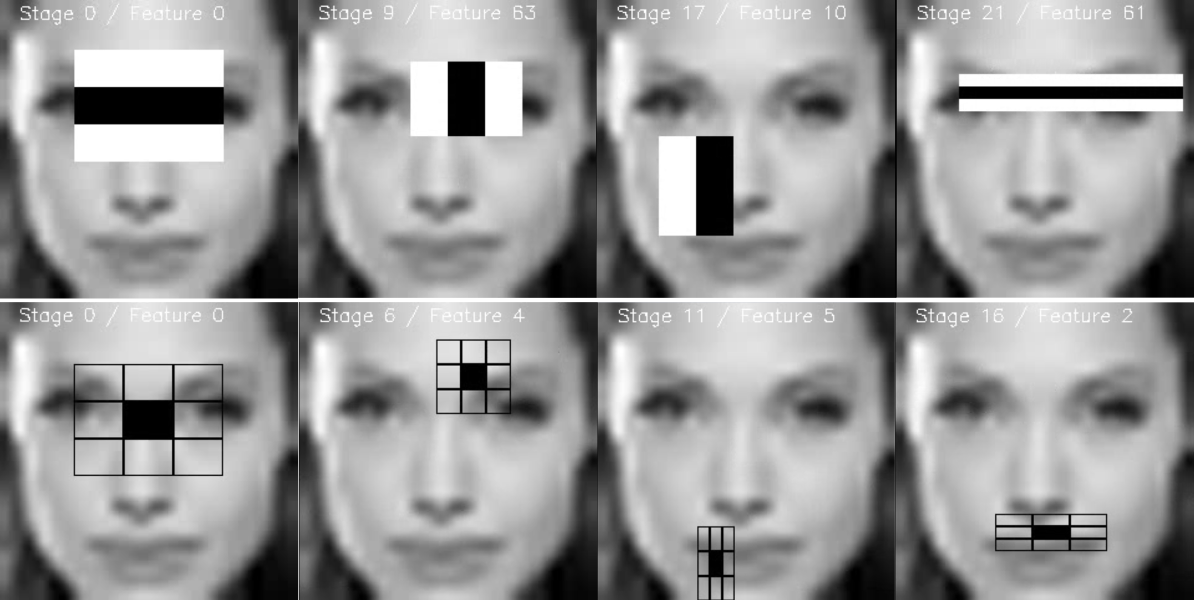
\includegraphics[width=\linewidth]{Bilder/haar-cascade.png}
\setcaptioncitation{ https://docs.opencv.org/master/dc/d88/tutorial\_traincascade.html}
\caption{haar features}
\label{fig: haar-features}
\end{figure}
Wie in der Grafik ebenfalls zu sehen ist, sind diese features alle samt rechteckig. Dies bietet die Möglichkeit die Berechnungen die gemacht werden müssen zu beschleunigen, indem Schritt zwei angewandt wird. die vorliegenden Bilder werden dabei in Integralbilder umgewandelt.  Diese werden im folgenden nicht genau expliziert, jedoch werden in Integralbildern vereinfacht gesagt in jedem Punkt des Bildes die Pixelsummen eines Rechteckes gehalten, das vom Ursprung bis zu dem jeweiligen Pixel aufgespannt wird. Bei einem Punkt (x,y) wird also das Rechteck (0,0) , (x,0), (0,y), (x,y) betrachtet.
\footcite[Vgl.][]{integral}
Nun können verschiedene Haar features selektiert werden. Das Problem dabei ist jedoch, dass diese für sich nicht sonderlich aussagekräftig sind. Beispielsweise ein Feature dass die Nasenflügel betrachtet ist nicht in der Lage ein Gesicht wirklich zu erkennen. Um deshalb ein aussagekräftiges Ergebnis zu erzielen werden die besten dieser sogenannten schwachen Klassifizierer zusammengefasst und trainiert,  zu einem starken Klassifizierer. Dieser Schritt beschreibt das Adaboost Training.
\footcite[Vgl.][]{willberger}
Diese Trainingsart benutzt nun den letzten Teil, das Kaskadieren von Klassifizieren. Im wesentlichen handelt es sich dabei um eine Methode die so schnell wie möglich falsche Bilder, also solche die nicht der gewünschten Klasse entsprechen, auszusortieren. Dabei wird in multiplen Stadien gearbeitet, in denen	 ein sich verschiebender Rahmen über das Bild gelegt wird, der wiederum die Größe des Zielbildes hat - Zum Beispiel eines Gesichtes, Auges, Mundes, etc. . Wenn nun der Rückgabewert für einen Ausschnitt den der Rahmen gerade umfasst negativ ist, wird der Rahmen weiter verschoben. Wenn das Ergebnis jedoch positiv ist, wird das Bild dem nächstem Stadium übergeben. 
\footcite[Vgl.][]{willberger}
Auf diese Weise können Gesichter mittels Haar Klassifizierung erkannt werden.
\subsubsection{Gesichtserkennungs Algorithmen}
Der Fisher Face Recognizer ist einer von drei Gesichtserkennungs Algortihmen die Opencv mit sich bringt. Einer seiner Gegenstücke ist der Eigenface Recognizer, auf dem der Fisher Face Recognizer partiell aufbaut. Aus diesem Grund wird zuerst die grundsätzliche Funktionsweise des Eigenface Algortihmus beleuchtet. Dieser Algorithmus bekommt einen Datensatz von verschiedenen Gesichtsbildern als Eingabeparameter. Der Eigenface Algortihmus stuft dabei verschiedene Gesichtskomponenten wichtiger ein als andere. zum Beispiel wenn mehr Varianz in den Trainingsdaten gegeben ist im Bereich der Nasen und Augen, und weniger im Bereich der Münder und Ohren,  wird der Algorithmus die Nasen und auch Augen als die sinnvolleren oder wichtigeren Komponenten erachten. Anhand dieser wichtigen Komponenten können dann verschieden Gesichter erkannt werden.
\footcite[Vgl.][]{Eigenface}
Das Problem dieses Algorithmus ist nun, dass viele Komponenten der Gesichter nicht mehr beachtet werden weil sie insgesamt eine zu niedrige Varianz aufgewiesen haben. Ein anderes Szenario wäre dass eine Komponente ohne Aussagekraft eine sehr große Varianz in den Trainingsdaten enthält. Z.B. Wenn in den Datensätzen eine hohe Varianz der jeweiligen Beleuchtung vorhanden ist, also wenn keine einheitlich Beleuchtung der Bilder vorhanden ist. Die Beleuchtung sagt per se nicht viel über ein Gesicht aus, aber der Eigenface Recognizer würde diese Komponente als sehr wichtig einstufen, was zu Fehlern führen kann.
\footcite[Vgl.][]{Fisherface}
Im Gegensatz zum Eigenface Recognizer arbeitet der Fisherface Algorithmus mit klassifizierten Daten. Daher ist er im Vergleich zum bereits explizierten Eigenface Ansatz ein supervised learning Algorithmus. Dieser supervised Algorithmus verfolgt ebenso den Ansatz dass aus dem Datensatz verschiedene Komponenten extrahiert werden, jedoch wird hierbei keine Gewichtung anhand der Varianz vorgenommen. Dadurch wird das zuvor beschriebene Problem teilweise aufgelöst. 
\footcite[Vgl.][How to fix this issue]{Eigenface}
Teilweise nur deshalb, weil ein Modell welches mit dem Fisherface Algorithmus trainiert wird und beispielsweise nur Bilder als Eingabewerte mit einer hohen Beleuchtung bekommt, auch nur solche Bilder korrekt bewerten kann. Wenn nun ein schlecht beleuchtetes Bild bewertet werden sollte, wird der Algorithmus an seine Grenzen kommen.
Dieses Problem kann unter anderem durch den dritten von Opencv angeboten Gesichtserkennungsalgorithmus ausgeglichen werden, dem sogenannten Local binary patterns histograms Recognizer. Ein weiterer Lösungsansatz wäre hingegen noch die Eingabedaten anzupassen, mit denen das resultierenden Modell trainiert wird. Darauf wird im folgenden Unterpunkt \pageref{subsec: Eingabe Daten} eingegangen. Da diese Vorbearbeitung das Problem der Beleuchtung ebenfalls löst, und dabei sogar noch weitere positive Aspekte für die Arbeit mit sich bringt, wird an dieser Stelle darauf verzichtet auf den Local binary patterns histograms Recognizer weiter einzugehen, und zum Nachlesen auf die Opencv Dokumenation verwiesen wird. 
\footcite[Vgl.][]{Recognizer} 
\subsection{Eingabe Daten}
\label{subsec: Eingabe Daten}
Wie im vorherigen Unterpunkt erwähnt kann das Modell ebenfalls dadurch beeinflusst werden wie der Eingabedatensatz aufgebaut ist. Dabei wird im Folgenden nicht auf den konkreten Datensatz eingegangen, sondern viel mehr auf die Anforderungen an die Beschaffenheit von diesem. Zunächst ist dabei zu beachten, dass es grundsätzlich einige Möglichkeiten gibt die Eingabedaten, in diesem Falle Bilder von Gesichtern, vorab zu bearbeiten. ein wesentlicher Aspekt dabei ist neben dem Anpassen der Bilder auf eine bestimmte Größe auch die Wahl der Farbdarstellung. Dabei geht es weniger darum ob beispielsweise die Bilder im RGB (Rot - Grün - Blau) oder HSV (Hue - Saturation - Value) Farbraum vorliegen, sondern um die generelle Zahl an Kanälen die Informationen von einem Bild beinhalten.
Beispielsweise wird bei einer klassichen RGB Darstellung auf drei Kanälen Informationen über das Bild gespeichert. 
\begin{figure}[h]
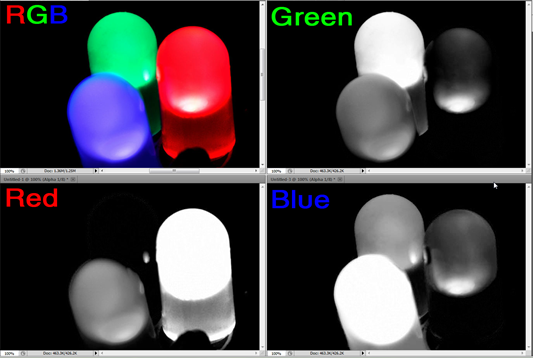
\includegraphics[width=\linewidth]{Bilder/RGB.png}
\setcaptioncitation{ https://www.howtogeek.com/wp-content/uploads/2011/02/sshot-74.png}
\caption{RGB Kanäle}
\label{fig: RGB}
\end{figure}
die obige Abbildung \ref{fig: RGB} zeigt wie die einzelnen Kanäle arbeiten. Informationen aus dem Grundbild die Rot erscheinen, werden im Roten Kanal besonders hell dargestellt. 
Ausschnitte aus der originalen Abbildung die blau erscheinen werden im blauen Kanal ebenso heller dargestellt. Analog zu den beiden Beispielen arbeitet ebenso der grüne Kanal.
 Werden die drei Kanäle wieder miteinander verbunden entsteht das Ausgangsbild. Der Vorteil solcher mehr kanaligen Formate ist, dass für das praktisch alle Informationen aus dem original Bild erhalten bleiben. Der Nachteil jedoch wird deutlich wenn die Farbe für den Anwendungsfall keine, oder eine geringe Rolle spielt. da in dieser Arbeit Emotionen anhand von Gesichtern erkannt werden soll, spielt die Farbe der Bilder selber eine untergeordnete Rolle, da diese keine nützlichen Informationen für das zu berechnende Modell enthält. Es wäre sogar kontraproduktiv, dadurch dass mehr Kanäle mit Informationen vorhanden sind, muss auch das Modell mehr Daten bekommen um zu lernen wie die Informationen aus diesen zu verstehen sind. Dies wird auch von dem sogenannten ''Fluch der Dimensionalität'' beschrieben. Auf den Anwendungsfall bezogen bedeutet dies nur, dass je mehr Eigenschaften ausgewertet werden sollen, desto mehr Daten zum Lernen müssen vorhanden sein. Um dem präventiv entgegenzuwirken, ohne in Verlegenheit zu geraten die Testdatensätze später erweitern zu müssen, können auch Bilder verwendet werden die auf weniger Kanäle an Informationen zurückgreifen. Sogenannte Grayscale oder Graustufen Bilder bieten hier den Vorteil, dass es nicht drei, sondern lediglich einen Farbkanal gibt. In diesem wird ein Wert pro Pixel gespeichert. Je höher dieser Wert, desto weißer der Pixel, je niedriger, desto schwärzer. Dieses Format eignet sich bestens für die Anwendung für das hier behandelte Modell, da keine wichtigen Informationen entfallen die in einer farbigen Version des Bildes vorhanden während sich aber die Anzahl der Daten verringert die benötigt werden um das Modell erfolgreich trainieren zu können. Dies erhöht wiederum die Chance das zuvor definierte should Kriterium zu erfüllen, welches besagt, dass die Wahrscheinlichkeit zur Erkennung der richtigen Emotion über 50\% liegen muss. 

\let\cleardoublepage\relax

\chapter{Stand-Alone Lösung mit Schwerpunkt OpenCV}
Während der weiteren Ausarbeitung des Konzeptes und der darauf basierenden Umsetzung sind letztendlich zwei verschiedene Lösungen entstanden. Aufgrund von Problemen die innerhalb des Entwicklungsprozesses im Zusammenhang mit dem Hardwarekonzept aufgetreten sind, konnte das Projekt so wie es geplant war nicht zu Ende gebracht werden. Da diese Lösung jedoch als Grundlage für die letztendlich finale Lösung diente, wird sowohl das Konzept als auch die Umsetzung der ersten Lösung genauer erläutert.

\section{Konzept}
Nachfolgend wird das in der Planungsphase entwickelte Konzept zur Emotionserkennung unter verschiedenen Aspekten wie der Architektur und der Kommunikation erläutert.

\subsection{Interaktionskonzept}
Von außen betrachtet, steht zuerst die Planung eines Interaktionskonzeptes an, in welcher Form der Nutzer die Möglichkeit hat, Input zur Verarbeitung zu liefern und an Output zu gelangen. Dem Anwender soll es möglich sein schnell und verständlich mit dem Produkt zu interagieren, deshalb ist eine geeignete Benutzeroberfläche mit zwei wesentlichen Interaktionsoptionen erforderlich, den aktuellen Video-Stream einer internen oder externen Kamera als Input zur Emotionsanalyse verwenden und das Ergebnis der analysierten Sequenzen ausgeben zu lassen. Um dies zu erreichen, soll die Bildbverarbeitungsbibliothek OpenCV verwendet werden, mit der sowohl der Zugriff auf alle verfügbaren Kameraeingabegeräte, als auch die Darstellung von Bildern und Text in einer grafischen Benutzeroberfläche (GUI) in Form eines Fensters möglich ist. Die vom Nutzer gelieferten Videosequenzen sollen entsprechend bearbeitet werden, um anschließend eine Emotion zu erkennen und den entstandenen Output an die durch OpenCV generierte Oberfläche weiterzugeben. In welcher konkreten Form der Output dem Nutzer letztendlich dargestellt wird, als Grafik, einfache Textausgabe oder audiovisuell ist noch zu entscheiden.\newline
Zusammenfassend kann man also sagen, dass der Nutzer aufgrund der Übersichtlichkeit und der Einfachheit halber lediglich mit der von OpenCV generierten Oberfläche interagiert und sich zu keinem Zeitpunkt mit den dahinterliegenden Komponenten der Emotionserkennung befassen muss.\newline
Es wird sich auch die Option vorbehalten, den Input über eine Client-Applikation an einen Server zu liefern und dem Nutzer den Output in der Client-Anwendung zurückzugeben, solange es den Anforderungen der benutzerfreundlichen Interaktionsmöglichkeit genügt. Um die Komplexität des Projektes weiterhin auf die wesentlichen Bestandteile der Emotionserkennung zu beschränken und nicht unnötig zu erhöhen, wird diese Möglichkeit jedoch vorerst nicht weiter berücksichtigt.

\subsection{Architektur}

\subsubsection{Programmierumgebung}
Aufgrund der Vorkenntnisse und Relevanz innerhalb des Studiums soll die Programmiersprache Python in aktuellster Version (3.6.9) vorrangig verwendet werden, jedoch kann unter gegeben Umständen auch die Programmiersprache C++ eingesetzt werden, was noch zu prüfen ist. Auf eine bestimmte IDE wie PyCharm, Emacs oder Visual Studio Code wird sich an dieser Stelle nicht festgelegt, da dies jedem Entwickler selbst zu überlassen ist. Diesbezüglich sind nur Einschränkungen aufgrund der gewählten Rechnerarchitektur und der Programmiersprache zu berücksichtigen.\newline
Zur Entwicklung einer Emotionserkennung sollen als grundlegende Komponenten die Programmbibliothek für Bildverarbeitung OpenCV und das Framework Tensorflow bzw. die Deep-Learning-Bibliothek Keras verwendet werden. Da das Einsatzgebiet von OpenCV in der Bildverarbeitung liegt, soll die Bibliothek dazu genutzt werden, den Input so zu verändern, dass dieser vom Modell zum trainieren oder vorhersagen einer oder mehrerer Emotionen verwendet werden kann. Für den wesentlichen Teil der Arbeit, das Entwickeln eines Modells, welches menschliche Emotion anhand eines Bildausschnittes von einem Gesichts erkennen kann, ist die Deep-Learning-Bibliothek Keras zu verwenden.

\subsubsection{Hardware}
Der Einfachheit halber wird als grundlegende Komponente ein handelsüblicher Laptop zum Entwickeln genutzt.  Außerdem wird dabei auf das OpenSource Betriebssystem Ubuntu 18.04.4 LTS in der 64-bit Variante zurückgegriffen. Als zugrunde liegende Ressourcen stehen ein 8 GigaByte Arbeitsspeicher sowie ein Intel Core i5-4210 Quadcore Prozessor mit einer Taktfrequenz von 4 x 2,60 GHz zur Verfügung. Des Weiteren kann die dedizierte Grafikkarte GeForce 820M mit einem Grafikkartenspeicher von 2046 MB verwendet werden. Der Festplattenspeicher von 500 GB kann im Umfang dieser Arbeit vernachlässigt werden, da es im Zusammenhang mit Gesichts- bzw. Emotionserkennung primär darauf ankommt, wie viel Rechenleistung zur Verfügung steht und nicht wie groß die Speicherkapazität des Laufwerks ist. Um das rechenintensive Trainieren des Modells zur Emotionserkennung in akzeptabler Zeit zu garantieren, soll die Rechenleistung des Prozessors und der Grafikkarte vollständig genutzt werden können.

\section{Umsetzung}
In diesem Kapitel wird die Umsetzung der auf dem entwickelten Konzept basierenden Lösung näher erläutert. Es handelt sich dabei um den Stand-Alone Laptop mit installiertem Ubuntu 18.04.4 LTS wobei der Input und der Output auf OpenCV GUIs basiert.

\subsection{Input GUI}
Als Einstieg in das Themengebiet Emotionserkennung bzw. Gesichtserkennung bietet sich an, sich zuerst mit den Grundlagen der Bildverarbeitung und den Grundlagen von OpenCV vertraut zu machen. Wie bereits im Konzept beschrieben, soll es dem User möglich sein, mithilfe der Webcam und einer grafischen Oberfläche, welche mit OpenCV programmiert wird, ein Bild als Input zu liefern. Wie man in Abbildung \ref{fig:Input GUI 1} sehen kann, wird im ersten Schritt die grafische Oberfläche erstellt und der Video Stream der Webcam in der Oberfläche angezeigt.
\lstinputlisting[style=custompython, caption=Code für GUI mit Video Stream der Webcam als Output]{Code/InputGUI1.py}
\begin{figure}[h]
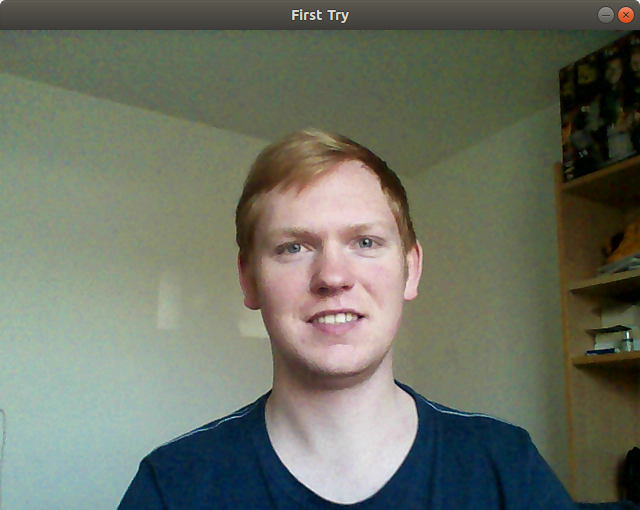
\includegraphics[width=\linewidth]{Bilder/InputGUI1.png}
\caption{GUI mit Video Stream der Webcam als Output}
\label{fig:Input GUI 1}
\end{figure}
Nachdem man nun auf den Video Stream der Webcam zugreifen und diesen wiedergeben kann, gilt es den relevanten Bildausschnitt, die sogenannte Region Of Interest (ROI), zu identifizieren. Da wir uns im Umfeld der Gesichts- und Emotionserkennung befinden, sind für uns alle Bereiche relevant, die ein menschliches Gesicht enthalten. Standardmäßig stellt OpenCV einige Modelle zur Objekterkennung zur Verfügung, welche problemlos genutzt werden können. Um nun ein vortrainiertes Modell zur Gesichtserkennung von OpenCV einzubinden, kann man folgende Zeile an den Anfang des Codes schreiben:\newline
\lstinputlisting[style=custompython, numbers=none, linerange=3-3, caption=Einbinden eines vortrainierten OpenCV-Modells zur Gesichtserkennung]{Code/InputGUI2.py}
Mithilfe der Methode \texttt{detectMultiScale} des eingebundenen Modells, können nun die Koordinaten sowie die Höhe und die Breite von jedem in dem Bild gefundenen Gesicht extrahiert werden. Aufgrund dieser Informationen können wir den bisherigen Code nun so erweitern, dass ein Rechteck um jedes gefundene Gesicht im Video Stream der Webcam gezeichnet wird und über die grafische Oberfläche ausgegeben wird. dies sieht dann folgendermaßen aus:\newline
\lstinputlisting[style=custompython, caption=Code für GUI mit Video Stream der Webcam und markierten Gesichtern als Output]{Code/InputGUI2.py}
Wie die durch den Code generiert grafischen Oberfläche aussieht, lässt sich der Abbildung \ref{fig:Input GUI 2} entnehmen.
\begin{figure}[h]
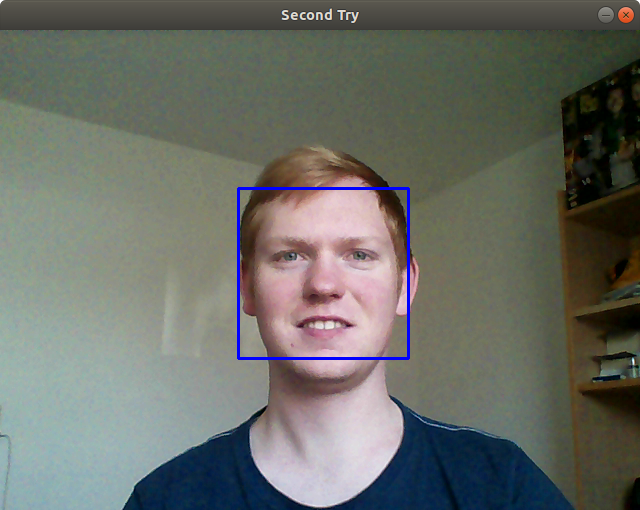
\includegraphics[width=\linewidth]{Bilder/InputGUI2.png}
\caption{GUI mit Video Stream der Webcam und markierten Gesichtern als Output}
\label{fig:Input GUI 2}
\end{figure}
Nun lässt sich noch darüber diskutieren, ob es weitere besonders zu berücksichtigende ROIs gibt. Im Zusammenhang mit Emotionen können unter anderem die Augen und der Mund eine besondere Rolle spielen, sodass nachfolgend einmal beispielhaft das Hinzufügen eines weiteren Modells zur Erkennung der Augen in jedem bereits entdeckten Gesicht:
\lstinputlisting[style=custompython, numbers=none, linerange=4-4, caption=Einbinden eines vortrainierten OpenCV-Modells zur Augenerkennung]{Code/InputGUI3.py}
Um nun alle Augen in einem Bild zu erkennen, kann nun wieder die Methode \texttt{detectMultiScale} des Modells genutzt werden. Dem nachfolgenden Codeschnipsel kann man nun entnehmen, wie um alle Augen, die sich in dem Bildausschnitt befinden in dem auch ein Gesicht erkannt wurde, ein grünes Rechteck gezeichnet wird.
\lstinputlisting[style=custompython, numbers=none, linerange=9-18, showspaces=false, autodedent, caption=Zeichnen von Rechtecken um alle erkannten Augen und Gesichter]{Code/InputGUI3.py}
Somit sind wir nun in der Lage, alle relevanten Bereiche zu identifizieren und zu markieren. Um diese relevanten Regionen nun als input zum Vorhersagen einer Emotion für ein Modell nutzen zu können, müssen die entsprechenden Bereiche jedoch ersteinmal abgespeichert werden. Um eine Vergleichbarkeit der Bilder untereinander und des zu testenden Bildes zu den trainierten Bildern zu gewährleisten, sollten diese alle das gleiche Format besitzen. Wie bereits in der Theorie erwähnt, ist es außerdem sinnvoll, entsprechende Ausschnitte nicht im Farbmodus abzuspeichern, sondern lediglich als Grayscale-Grafik. Erweitert man den bereits entstandenen Code erneut um die erleuterten Aspekte, sieht dies so aus:
\lstinputlisting[style=custompython, caption=Code für GUI mit Video Stream der Webcam und markierten Gesichtern und Augen als Output]{Code/InputGUI3.py}
Das daraus resultierende Ergebnis kann man der Abbildung \ref{fig:Input GUI 3} entnehmen.
\begin{figure}[h]
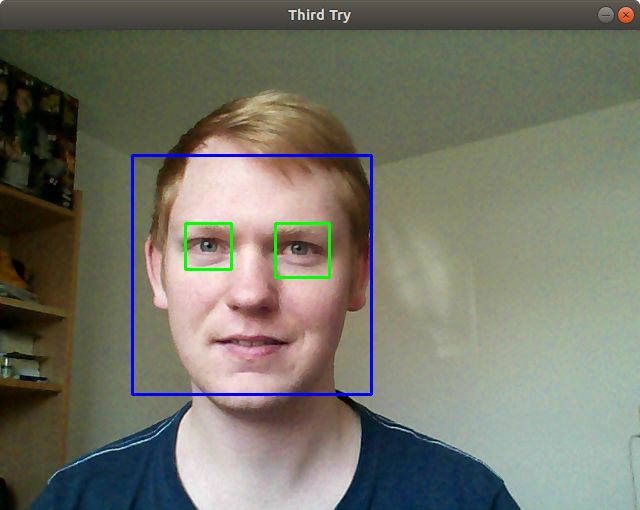
\includegraphics[width=\linewidth]{Bilder/InputGUI3.png}
\caption{GUI mit Video Stream der Webcam und markierten Gesichtern und Augen als Output}
\label{fig:Input GUI 3}
\end{figure}
Somit ist es dem Nutzer möglich, schnell und unkompliziert Bilder mit der Webcam zu machen und dort enthaltene Gesichter so zu speichern, dass sie als Input zum Vorhersagen einer Emotion genutzt werden können.

\subsection{Dataset}
Zum Trainieren eines Modells zur Emotionserkennung, wird das sogenannte Cohn-Kanade Dataset zur Analyse von Emotionen verwendet.\footcite[Vgl.][]{CK} In dem verwendeten Dataset sind ca. 10000 Grayscale-Bilder enthalten, welche die in \ref{tab:ckemotions} zu sehenden Emotionen:
\begin{table}[h]
\centering
\begin{tabular}[t]{l|c}
Emotion & N \\
\hline
Anger & 45 \\
Contempt & 18 \\
Disgust & 59 \\
Fear & 25 \\
Happy & 69 \\
Sadness & 28 \\
Surprise & 83 \\
\hline
\end{tabular}
\caption{Emotionen mit jeweiliger Anzahl an Bildern}
\label{tab:ckemotions}
\end{table}
Es fällt auf, dass sich die dargestellte Anzahl von ca. 325 nutzbaren Bilder stark von der bereits erwähnten Anzahl von 10000 Bildern unterscheidet. Dies liegt daran, dass das Dataset ursprünglich für die Analyse von Emotionen und nicht direkt für die Emotionserkennung entwickelt wurde. Was das kann genau hast, wird durch die Abbildung \ref{fig:Disgust} verdeutlicht.
\begin{figure}[h]
	\begin{minipage}[b]{.2\linewidth} % [b] => Ausrichtung an \caption
		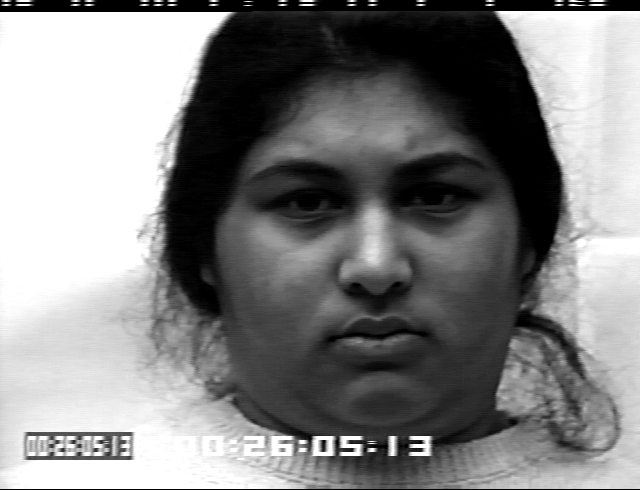
\includegraphics[width=\linewidth]{Bilder/Disgust1.png}
	\end{minipage}
	\hspace{.025\linewidth}% Abstand zwischen Bilder
	\begin{minipage}[b]{.2\linewidth} % [b] => Ausrichtung an \caption
		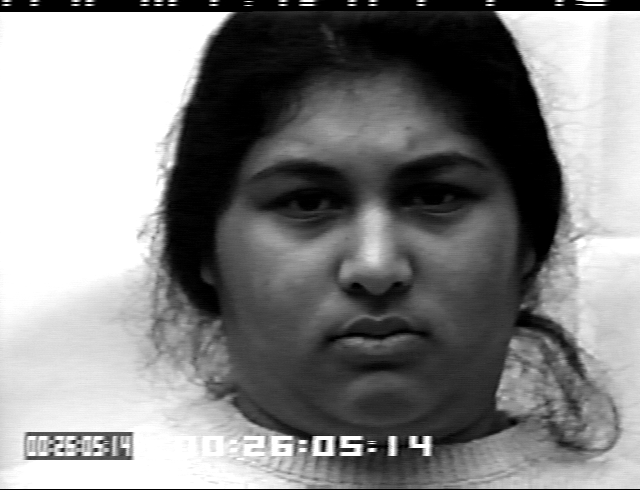
\includegraphics[width=\linewidth]{Bilder/Disgust2.png}
	\end{minipage}
	\hspace{.025\linewidth}% Abstand zwischen Bilder
	\begin{minipage}[b]{.2\linewidth} % [b] => Ausrichtung an \caption
		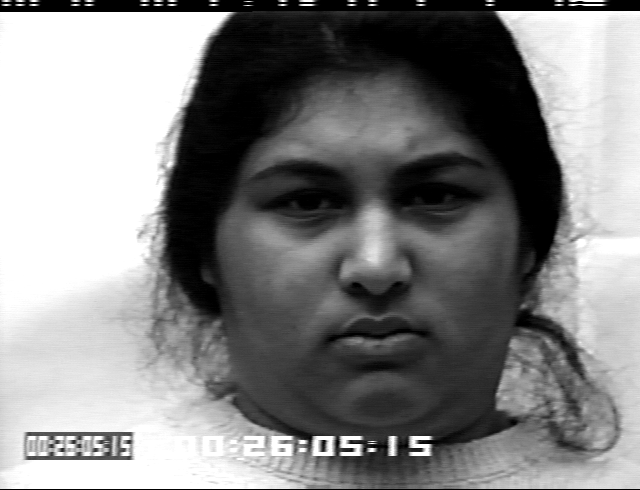
\includegraphics[width=\linewidth]{Bilder/Disgust3.png}
	\end{minipage}
	\hspace{.025\linewidth}% Abstand zwischen Bilder
	\begin{minipage}[b]{.2\linewidth} % [b] => Ausrichtung an \caption
		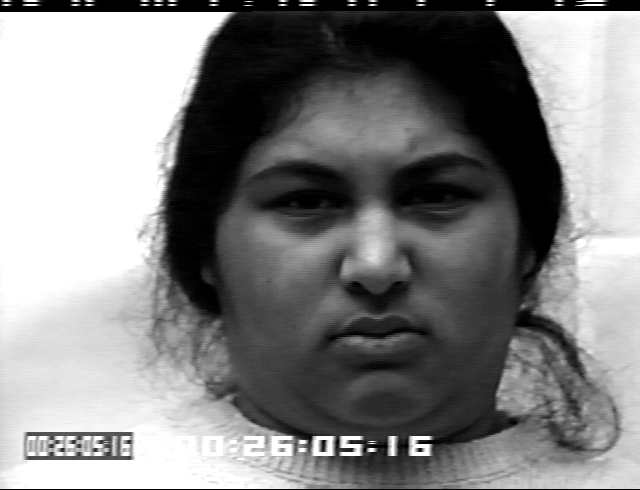
\includegraphics[width=\linewidth]{Bilder/Disgust4.png}
	\end{minipage}
	\newline
	\begin{minipage}[b]{.2\linewidth} % [b] => Ausrichtung an \caption
		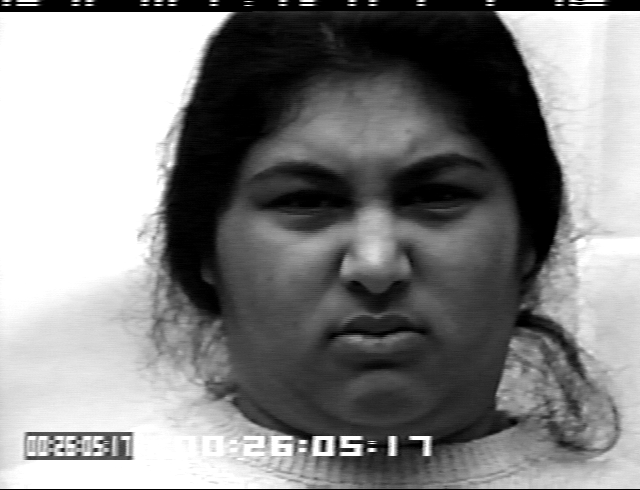
\includegraphics[width=\linewidth]{Bilder/Disgust5.png}
	\end{minipage}
	\hspace{.025\linewidth}% Abstand zwischen Bilder
	\begin{minipage}[b]{.2\linewidth} % [b] => Ausrichtung an \caption
		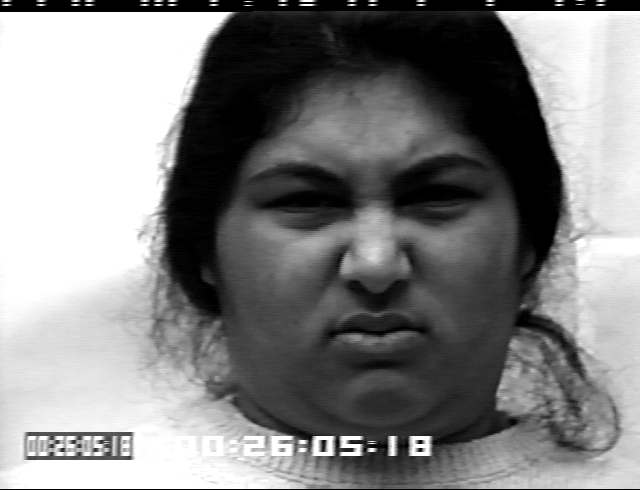
\includegraphics[width=\linewidth]{Bilder/Disgust6.png}
	\end{minipage}
	\hspace{.025\linewidth}% Abstand zwischen Bilder
	\begin{minipage}[b]{.2\linewidth} % [b] => Ausrichtung an \caption
		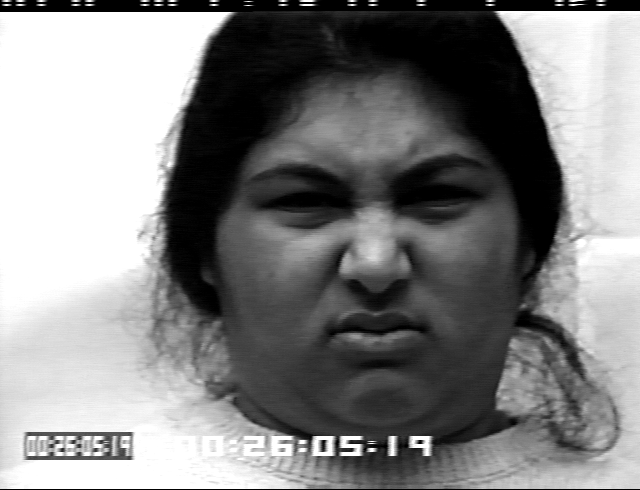
\includegraphics[width=\linewidth]{Bilder/Disgust7.png}
	\end{minipage}
	\hspace{.025\linewidth}% Abstand zwischen Bilder
	\begin{minipage}[b]{.2\linewidth} % [b] => Ausrichtung an \caption
		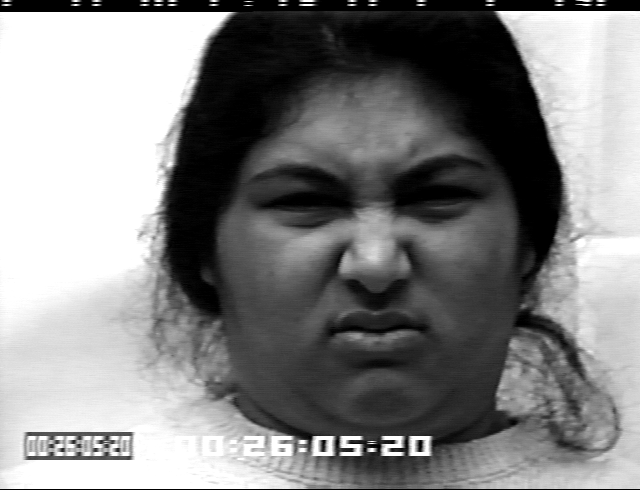
\includegraphics[width=\linewidth]{Bilder/Disgust8.png}
	\end{minipage} 
	\newline
	\begin{minipage}[b]{.2\linewidth} % [b] => Ausrichtung an \caption
		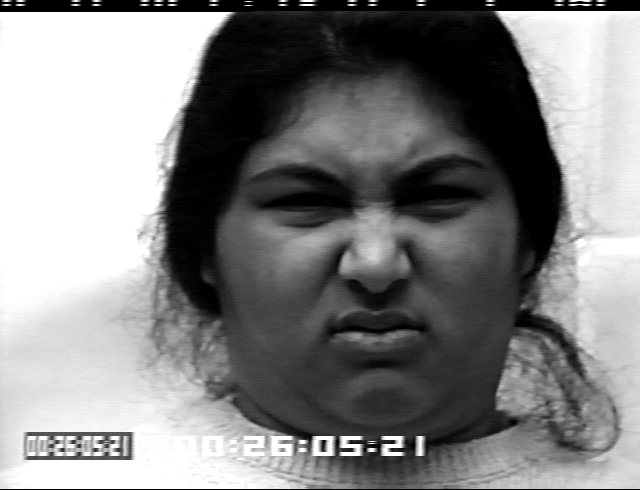
\includegraphics[width=\linewidth]{Bilder/Disgust9.png}
	\end{minipage}
	\hspace{.025\linewidth}% Abstand zwischen Bilder
	\begin{minipage}[b]{.2\linewidth} % [b] => Ausrichtung an \caption
		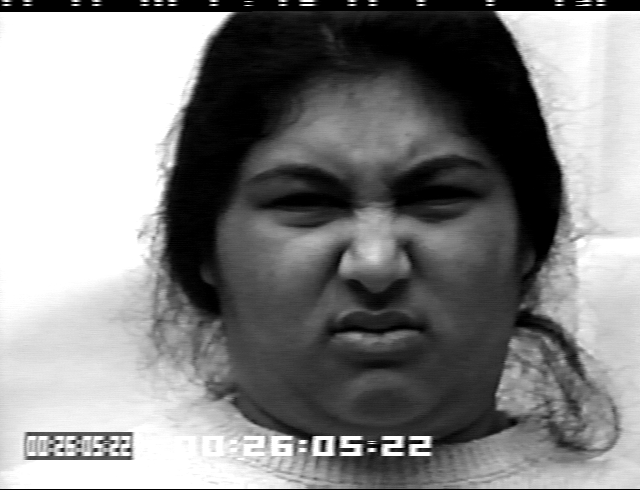
\includegraphics[width=\linewidth]{Bilder/Disgust10.png}
	\end{minipage}
	\hspace{.025\linewidth}% Abstand zwischen Bilder
	\begin{minipage}[b]{.2\linewidth} % [b] => Ausrichtung an \caption
		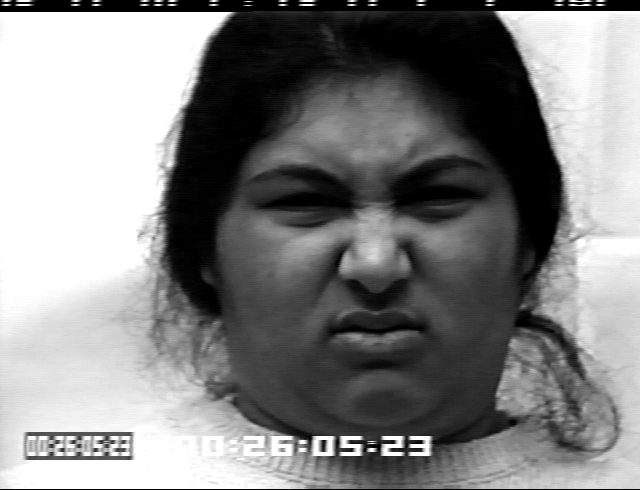
\includegraphics[width=\linewidth]{Bilder/Disgust11.png}
	\end{minipage}
	\caption[t]{Emotionsverlauf von Neutral zu Disgust}
	\label{fig:Disgust}
\end{figure}

Jeder Datensatz beinhaltet mehrere Bilder, die den Verlauf einer Emotion von Neutral bis hin zur Emotion darstellen. Da dieser Verlauf für die Emotionserkennung allenfalls für die Klassifizierung innerhalb der jeweiligen Emotion relevant wäre und somit im Umfang dieser Arbeit nicht betrachtet wird, wird nur das jeweils letzte Bild dieses Verlaufs, also die vollständig ausgeprägte Emotion, zum Trainieren des Modells genutzt. Somit ergibt sich der Unterschied von der Anzahl der jeweils letzten Bilder der Verläufe, ca. 325, und der Anzahl der Gesamtbilder aller Verläufe, ca. 10000.
Zur Verzeichnisstruktur des Datasets kann sagen, dass es grundsätzlich zwei verschiedene Ordner gibt. In einem Ordner befinden sich alle Bilder, also die Verläufe der Emotionen und in dem anderen befinden sich mit der gleichen Struktur die dazugehörigen Emotionen. Stellt man die Struktur der beiden Ordner beispielhaft als Verzeichnisbaum dar, sieht dies folgendermaßen aus:
\setlength{\DTbaselineskip}{20pt}
\DTsetlength{1em}{1.5em}{0.2em}{1pt}{4pt}
\renewcommand*\DTstylecomment{\rmfamily\color{commentgreen}\textsc}
\renewcommand*\DTstyle{\ttfamily\textcolor{red}}
\begin{figure}
\begin{minipage}[b]{.5\linewidth}
\dirtree{%
.1 images.
.2 S005\DTcomment{Person 1}.
.3 001.
.2 S010\DTcomment{Person 2}.
.3 001.
.3 002.
.3 003.
.2 S011\DTcomment{Person 3}.
.3 001.
.3 002.
.2 S014\DTcomment{Person 4}.
.3 001.
.3 002.
.3 003.
.3 004.
.3 005.
.2 \ldots.
}
\end{minipage}
\begin{minipage}[b]{.5\linewidth}
\dirtree{%
.1 emotions.
.2 S005\DTcomment{Person 1}.
.3 001.
.2 S010\DTcomment{Person 2}.
.3 001.
.3 002.
.3 003.
.2 S011\DTcomment{Person 3}.
.3 001.
.3 002.
.2 S014\DTcomment{Person 4}.
.3 001.
.3 002.
.3 003.
.3 004.
.3 005.
.2 \ldots.
}
\end{minipage}
\caption{fig:Test}
\end{figure}
Wie man den Verzeichnisbäumen entnehmen kann, ist die Struktur in beiden Ordnern identisch. In der ersten Ebene befinden sich Ordner jeweils mit 'S' aufgeteilt nach Personen. Innerhalb jeder dieser Personenordner gibt es einen oder mehrere weitere Ordner. Diese Ordner auf der 2. Ebene sind dreistellig aufsteigend numeriert und beinhalten jeweils einen Emotionsverlauf. Im Sachzusammenhang bedeutet dies, dass jede Person eine oder mehrere verschiedene Emotionsverläufe darstellt. Die Syntax der Dateinamen in den aufsteigend numerierten Ordner, die letztendlich den Emotionsverlauf beinhalten, ist \texttt{<Personenordner>\_<Emotionsverlaufsordner>\_<Pos. im Verlauf>.png} wobei die Position im Verlauf 8-stellig ist. Nimmt man die in Abbildung \ref{fig:Disgust} als Grundlage, könnten die einelnen Dateinamen zu den Bildern wie im Verzeichnisbaum \ref{fig:Tree Emotionsverlauf} aussehen.
\begin{figure}
\dirtree{%
.1 images.
.2 S005\DTcomment{Person 1}.
.3 001\DTcomment{Emotionsverlauf 1}.
.4 S005\_001\_00000001.png.
.4 S005\_001\_00000002.png.
.4 S005\_001\_00000003.png.
.4 S005\_001\_00000004.png.
.4 S005\_001\_00000005.png.
.4 S005\_001\_00000006.png.
.4 S005\_001\_00000007.png.
.4 S005\_001\_00000008.png.
.4 S005\_001\_00000009.png.
.4 S005\_001\_00000010.png.
.4 S005\_001\_00000011.png.
.2 \ldots.
}
\caption{Struktur Emotionsverlauf}
\label{fig:Tree Emotionsverlauf}
\end{figure}
Aus der dargestellten Struktur des Ordners in dem sich sämtliche Bilder befinden und den jeweiligen Dateinamen lassen sich keinerlei Rückschlüsse auf die dargestellten Emotionen ziehen. Um herauszufinden welche Emotion durch welchen Emotionsverlauf dargestellt wird, muss man in das entsprechende Verzeichnis in dem Ordner mit den gelabelten Emotionen wechseln. Dort befindet sich dann eine Textdatei, die den selben Dateinamen hat, wie das letzte Bild aus dem dazugehörigen Emotionsverlauf. In dieser Datei befindet sich dann eine Fließkommazahl, die für die jeweilige Emotion in Tabelle \ref{tab:ckemotions} steht. Um nun herauszufinden welche Emotion durch den in \ref{fig:Tree Emotionsverlauf} dargestellt wird, schaut man in das Verzeichnis \texttt{emotions/S005/001/}, in dem sich die Datei \texttt{S005\_001\_00000011.txt} befindet. In dieser Datei würde dann \texttt{3.0000000e+00} stehen, was sich gemäß der Tabelle mit \texttt{Disgust} gleichsetzen lässt.\newline
Um später ein vernüftiges superviesed learning auf Grundlage des Dataset durchzuführen, wird eine eigene Verzeichnisstruktur erstellt, die jedes letzte Bild eines Emotionsverlaufs sortiert nach Emotion beinhaltet. Der folgenden Code automatisiert das überarbeiten und sortieren des Datasets und erweitert dieses um die Emotion \texttt{Neutral}, da jedes erste Bild eines Emotionsverlaufs als neutrale Ausgangslage dient.
\lstinputlisting[style=custompython, caption=Dataset sortieren und überarbeiten]{Code/OrganizingTheDataset.py}
Das überarbeitete und sortierte Dataset, welches nun als neue Grundlage für die Stand-Alone Lösung dient, sieht dann so aus:
\begin{figure}
	\dirtree{%
	.1 sorted\_set.
	.2 anger.
	.3 1.png.
	.3 2.png.
	.3 \ldots.
	.2 contempt.
	.3 1.png.
	.3 2.png.
	.3 \ldots.
	.2 disgust.
	.3 1.png.
	.3 2.png.
	.3 \ldots.
	.2 fear.
	.3 1.png.
	.3 2.png.
	.3 \ldots.
	.2 happy.
	.3 1.png.
	.3 2.png.
	.3 \ldots.
	.2 neutral.
	.3 1.png.
	.3 2.png.
	.3 \ldots.
	.2 sadness.
	.3 1.png.
	.3 2.png.
	.3 \ldots.
	.2 surprise.
	.3 1.png.
	.3 2.png.
	.3 \ldots.
	}
\caption{Struktur überarbeitetes Dataset}
\label{fig:Tree Sorted Set}
\end{figure}

\subsection{Training}
OpenCV stellt verschiedene Klassifizierer zur Verfügung, jedoch wird sich in diesem Abschnitt immer auf das Supervised Learning des FisherFaceRecognizer bezogen, welcher mit dem im vorherigen Schritt präparierten Dataset trainiert wird. Da das Dataset schon sortiert und vorbereitet wurde, ist es nun sehr leicht eine Methode zu schreiben, die ein Array mit Trainingsdaten und ein Array mit den zugehörigen Labels liefert. Aufgrund der Verzeichnisstruktur des Datasets kann man über alle Emotionsordner iterieren und alle Grayscale-Bilder in das Array mit den Trainingsdaten einlesen und die jeweilige Emotion in das Array mit den Labels einlesen. Dabei ist jedoch zu beachten, dass die Labels Integer-Werte aufsteigend mit 0 beginnend sein müssen. Das heißt, die Ordnernamen, welche die Emotionen als Text sind, müssen in Integer-Werte konvertiert werden, indem man z.B. den jeweiligen Index in dem Emotions-Array \lstinputlisting[style=custompython, numbers=none, linerange=5-5, caption=Emotions-Array]{Code/ClassifierHandler.py} nimmt. Setzt man dies um, entsteht folgender Code:
\lstinputlisting[style=custompython, numbers=none, linerange=8-17, caption=Trainingsdaten als Arrays extrahieren]{Code/ClassifierHandler.py}
Da wir nun die erforderlichen Arrays mit Trainingsdaten und Labeln erzeugen können, beschäftigen wir uns als nächstes mit dem zu trainierenden Klassifizierer, dem sogenannten FisherFaceRecognizer. Im folgenden werden zwei Methoden dargestellt, mit denen dieser erzeugt und trainiert werden kann.
\lstinputlisting[style=custompython, numbers=none, linerange=19-24, caption=Methoden zum Erstellen und Trainieren eines FisherFaceRecognizer]{Code/ClassifierHandler.py}
Da nun alle erforderlichen Einzelschritte definiert sind, können wir diese nun zusammenfügen. \lstinputlisting[style=custompython, numbers=none, linerange=55-57, caption=Erstellen und Trainieren eines FisherFaceRecognizer]{Code/ClassifierHandler.py}
Wie dem Code zu entnehmen ist, stellt die \texttt{FisherFaceRecognizer}-Klasse die Methoden \texttt{create()} und \texttt{train(InputArray data, InputArray labels)} zur Verfügung, sodass der Großteil der Komplexität des gesamten Trainingsprozesses bei dem Vorbereiten des Datasets liegt.

\subsection{Testing}
Das Testen des im vorherigen Schritt trainierten Modells kann aufgrund der Vorarbeit ebenfalls sehr schnell implementiert werden. Aufgrund der wie sich später herausstellte sehr geringen Datengrundlage und der Should-Anforderung gemäß MoSCoW Priorisierung, dass die Wahrscheinlichkeit zu Erkennung der richtigen Emotion über 50\% liegen soll, wird anstatt der üblichen Aufteilung des Datasets in Trainings- und Testdaten das komplette Dataset als Trainingsdaten genutzt. Daraus ergibt sich dann, dass ein anderes Verfahren zum Testen des Klassifiziers gefunden werden muss. Somit wird zum Testen des Modells eine grafische Oberfläche erstellt, die im speziellen als Echtzeitanalyse der Emotionen fungiert. Hierzu kann ein Großteil des Codes genutzt werden, der als Vorarbeit im Bereich der Input GUI implementiert wurde. Der Ablauf eines konkreten Tests ist dann das Starten der Oberfläche, welche den Video Stream der Webcam ausgibt und gleichzeitig jedes Einzelbild vom Modell analysieren lässt. Dies geschieht wie ebenfalls bereits beschrieben durch das Ausschneiden des Gesichtes und das anschließende konvertieren in das Grayscaleformat sowie daraufhin das wesentliche Vorhersagen einer Emotion. Das Gesicht wird dann mit einem Rechteck markiert und darüber wird die vorhergesagte Emotion ausgegeben. Verändert man den Code der Input GUI nur geringfügig und erweitert ihn um das Vorhersagen der Emotion und das Schreiben der vorhergesagten Emotion auf den Output Video Stream, dann erhält man folgendes Ergebnis:
\lstinputlisting[style=custompython, numbers=none, linerange=26-50, caption=Klassifizierer mit der Input GUI testen]{Code/ClassifierHandler.py}

\subsection{Optimierung der Lösung}
Durch das Testen des Modells konnte festgestellt werden, dass trotz der vergrößerten Menge an Daten zum Trainieren, die Genauigkeit der Vorhersagen deutlich unter 50\% liegt. Aufgrund dieser Tatsache wird versucht, den Trainingsprozess zu optimieren. Die Möglichkeiten zum komplexen Konfigurieren eines Modells in OpenCV sind begrenzt, so dass das Konfigurieren eines Modells, welches wesentlich mehr Features der Emotion analysiert als zuvor, erschwert wird. Außerdem würde sich dann die Tatsache bemerkbar mahcen, dass OpenCV keine Möglichkeit bietet, die  Rechenleistungen der CPU und der GPU zu kombinieren. Daraus würde sich ein sehr langwieriger Trainingsprozess ergeben, was nicht mehr den Anforderungen entspricht. Daher wird zunächst versucht, den Prozess in eine extra dafür vorgesehene Bibiliothek auszulagern, wobei die Entscheidung auf die Keras-API des Tensorflow-Frameworks gefallen ist. Auf die genaue funktionsweise von Keras wird in einem späteren Kapitel näher eingegangen. An dieser Stelle bleibt dann nur noch zu bemerken, dass die Installation von Keras und das Einbinden benötigter Komponenten erfolgreich durchgeführt werden konnte, jedoch die Ausführen der benötigten Komponenten wegen einer nicht unterstützten Prozessorarchitektur bzw. eines nicht unterstützten Chipsets nicht möglich war. Aufgrund der benötigten Ressourcen und der mit Tensorflow kompatiblen Architektur wurde sich deshalb für eine Server-Client-Architektur entschieden, wobei der Server in einer uns zur Verfügung gestellten Cloudumgebung gehostet wird.

\chapter{Server-Client Lösung}
Basierend auf den Erfahrungen, die während des Entwicklunsprozesses der Stand-Alone Lösung gewonnen werden konnten, werden das Konzept und dementsprechend auch die Umsetzung überarbeitet und optimiert. Nachfolgend wird die damit finale Lösung genauer erläutert.

\section{Konzept}
Die Interaktionsmöglichkeiten, die der Nutzer haben soll, bleiben unverändert. Der Übersichtlichkeit halber soll ausschließliche mit einer mithilfe von OpenCV generierten grafischen Oberfläche interagiert werden. Die Wesentlichen Änderungen beschränken sich auf die Systemarchitektur, insbesodere auf die Programmierumgung.

\subsection{Programmierumgebung}
Zusätzlich zu den bereits erwähnten Gründen für die Entscheidung der Programmiersprache Python ist noch die Wiederverwendbarkeit der bisher entwickelten Lösung zu nennen. Um den Anforderungen bezüglich der dem Projekt zur Verfügung stehenden Zeit gerecht zu werden, wird weiterhin die Programmiersprache Python verwendet, da so der bisher implementierte Code als Grundlage dienen kann und die neue Lösung darauf aufbauend entwickelt werden kann.
Außerdem stellt sich nun die Frage, mit welcher Entwicklungsumgebung gearbeitet wird. Da nun auf einer Cloud-Infrastruktur entwickelt wird, sind die reinen grafischen Umgebungen wie Visual Studio Code oder PyCharm nicht zu empfehlen. Aufgrund vieler Vorteile, die dem entsprechenden Kapitel zu entnehmen sind und der ebenfalls bereits erwähnten Relevanz innerhalb des Studiums wird zum weiteren Entwickeln die Open-Source Webapplikation Jupyter Notebook verwendet. Da über das Webinterface insbesondere das Debugging vereinfacht wird, kann vor allem der Entwicklungsprozess signifikant beschleunigt werden. Der Einheitlichkeit halber wird die Clientanwendung ebenfalls mithilfe von Jupyter Notebook entwickelt, wobei diese in der finalen Version durch minimale Anpassungen auch problemlos ohne Jupyter Notebook ausführbar gemacht werden kann. OpenCV, die Programmbibliothek für Bildverarbeitung und Keras, die Deep-Learning-Bibliothek, werden weiterhin für die bereits beschriebenen Zwecke verwendet.

\subsection{Hardware}


\section{Umsetzung}
Trotz der aufgetretenen Komplikationen bei der Entwicklung einer Stand-Alone Lösung muss an dieser Stelle erwähnt werden, dass große Teile, gerade im Bereich des Inputs und Outputs wiederverwendet werden. Die auf Grundlage der Stand-Alone Version entwickelte Server-Client Lösung wird nachfolgend genauer erläutert.

\subsection{Dataset}
Im Zuge der vertieften Recherche nach Keras und der direkten Verwendung im Bereich Gesichts- und Emotionserkennung wurde ein besseres Dataset gefunden, als bisher verwendet wurde. Das Dataset gehört zu einer Open-Source Facial Expression Recognition auf Kaggle.\footcite[Vgl.][]{FER-Challenge} Kaggle ist eine Online-Community deren Hauptzweck es ist, Data-Science-Wettbewerbe auszuschreiben, an denen jeder interessierte teilnehmen kann. Außerdem ermöglicht die Platform Datensätze zu finden und zu veröffentlichen und ggf. Modelle auszuprobieren oder ebenfalls zu veröffentlichen. Vereinfacht kann mann sagen, dass Kaggle ein virtueller Treffpunkt für Data-Scientists in den Bereichen Maschinelles Lernen und KI-Entwicklung ist.\newline
Betrachten wir nun das im Projekt verwendete Dataset.
Das Dataset umfasst 35887 Datensätze, die allesamt gelabelt sind. Dabei wird das Set in Trainingsdaten, Public-Testdaten und Private-Testdaten unterteilt, wobei 80\% aller Werte auf das Trainingsset entfallen und jeweils 10\% auf die Testsets. Die Unterteilung der Testdaten in Public und Private ist dabei nur im direkten Zusammenhang mit dem Kaggle-Wettbewert von Relevanz, da ein Set zum Testen des Modells für die Entwickler selbst ist und das Andere, um einen Sieger der Challenge auszumachen. Da wir mit unserem Modell nicht an der Facial Emotion Recognition Challenge teilnehmen, können wir die beiden Testsets zu einem großen zusammenfassen. Damit erhalten wir 28709 Datensätze zum Trainieren des Modells und 7178 Datensätze zum Testen. Aufgrund der Menge an Daten werden diese nicht wie beim anderen Dataset in einer Ordnerstruktur mit entsprechend vielen Bilddateien zur Verfügung gestellt, sondern als Comma-Separated-Values (.csv). Dabei handelt es sich um eine Art Tabelle, deren Struktur beispielhaft der Tabelle \ref{tab:FER2013} zu entnehmen ist.
\begin{table}[h]
\centering
\begin{tabular}[t]{c|l|c}
emotion & pixels & Usage \\
\hline
0 & 70 80 82 72 58 58 60 63 54 58 60 48 89 115 121 119 115 110 98 ... & Training \\
0 & 151 150 147 155 148 133 111 140 170 174 182 154 153 164 173 178 ... & Training \\
2 & 231 212 156 164 174 138 161 173 182 200 106 38 39 74 138 161 ... & Training \\
4 & 24 32 36 30 32 23 19 20 30 41 21 22 32 34 21 19 43 52 13 26 40 ... & Training \\
6 & 4 0 0 0 0 0 0 0 0 0 0 0 3 15 23 28 48 50 58 84 115 127 137 142 ... & Training \\
2 & 55 55 55 55 55 54 60 68 54 85 151 163 170 179 181 185 188 188 ... & Training \\
4 & 20 17 19 21 25 38 42 42 46 54 56 62 63 66 82 108 118 130 139 ... & Training \\
3 & 77 78 79 79 78 75 60 55 47 48 58 73 77 79 57 50 37 44 56 70 80 ... & Training \\
0 & 254 254 254 254 254 249 255 160 2 58 53 70 77 76 75 78 68 18 32 ... & PublicTest \\
0 & 170 118 101 88 88 75 78 82 66 74 68 59 63 64 65 90 89 73 80 80 ... & PrivateTest \\
\hline
\end{tabular}
\caption{Struktur des CSV-Datasets der FER-Challenge}
\label{tab:FER2013}
\end{table}
Die Spalte \texttt{emotion} kann dabei Werte von 0 bis 6 annehmen, wobei sich insgesamt 7 verschiedene Werte ergeben, die den Emotionen entsprechend der Tabelle \ref{tab:feremotions} zugeordnet werden können. Außerdem werden in der Tabelle die absoluten und relativen Häufigkeiten der Emotionswerte dargestellt, da diese für spätere Optimierungen relevant sind.
\begin{table}[h]
\centering
\begin{tabular}[t]{c|c|c|c}
Wert & Emotion & $H_n$ & $h_n$ \\
\hline
0 & Angry & 4953 & 13,80\% \\
1 & Disgust & 547 & 1,52\% \\
2 & Fear & 5121 & 14,27\% \\
3 & Happy & 8989 & 25,05\% \\
4 & Sad & 6077 & 16,93\% \\
5 & Surprise & 4002 & 11,15\% \\
6 & Neutral & 6198 & 17,27\% \\
\hline
\end{tabular}
\caption{Zuordnung und Häufigkeiten der Emotionen}
\label{tab:feremotions}
\end{table}
\begin{figure}[h]
\begin{tikzpicture}
	\begin{axis}[
	  ybar,
	  axis x line = bottom,
	  enlarge x limits = .1,
	  bar width=20pt,
	  nodes near coords,
	  symbolic x coords ={Angry, Disgust, Fear, Happy, Sad, Surprise, Neutral},
	  x tick label style={rotate=45,anchor=north east},
	  title = {Häufigkeitsverteilung der Emotionen}
	  ]
	  \addplot[fill=blue] coordinates {
		(Angry,4953)
		(Disgust,547)
		(Fear,5121)
		(Happy,8989)
		(Sad,6077)
		(Surprise,4002)
		(Neutral,6198)
	  };
	\end{axis}
  \end{tikzpicture}
\end{figure}
Betrachten wir nun die anderen Spalten. In der Spalte \texttt{pixels} befinden sich die eigentlichen Bilddaten als Pixelwerte, die lediglich mit einem Leerzeichen getrennt in einem String dargestellt werden. In Tabelle \ref{tab:FER2013} wird nur ein kleiner Ausschnitt der insgesamt 2304 Pixelwerte pro Datensatz angezeigt, wobei jedes Pixel Werte von 0 bis 255 annehmen kann. Die Anzahl von 2304 Pixeln ergibt sich durch die Länge und die Breite der Bilder von jeweils 48 Pixel mal 48 Pixel. Bevor man die Bilddaten in Form des Strings aus Pixeln für das Modell nutzen kann, müssen diese erst entsprechend formatiert und ungeformt werden, aber dazu später mehr.  
Die letzte der Tabelle zu entnehmende Information befindet sich in der Spalte \texttt{Usage}. Dort wird jedem Datensatz zugeordnet, ob er im Zuge des Wettbewerbes zum Trainieren, zum privaten Testen oder zum öffentlichen Testen verwendet wird.

\subsection{Modell}
Nachfolgend wird das für die Emotionserkennung erstellte Modell mit den jeweils einzelnen Layern näher erläutert und \ref{fig:Model Summary}

\begin{figure}[H]
\center
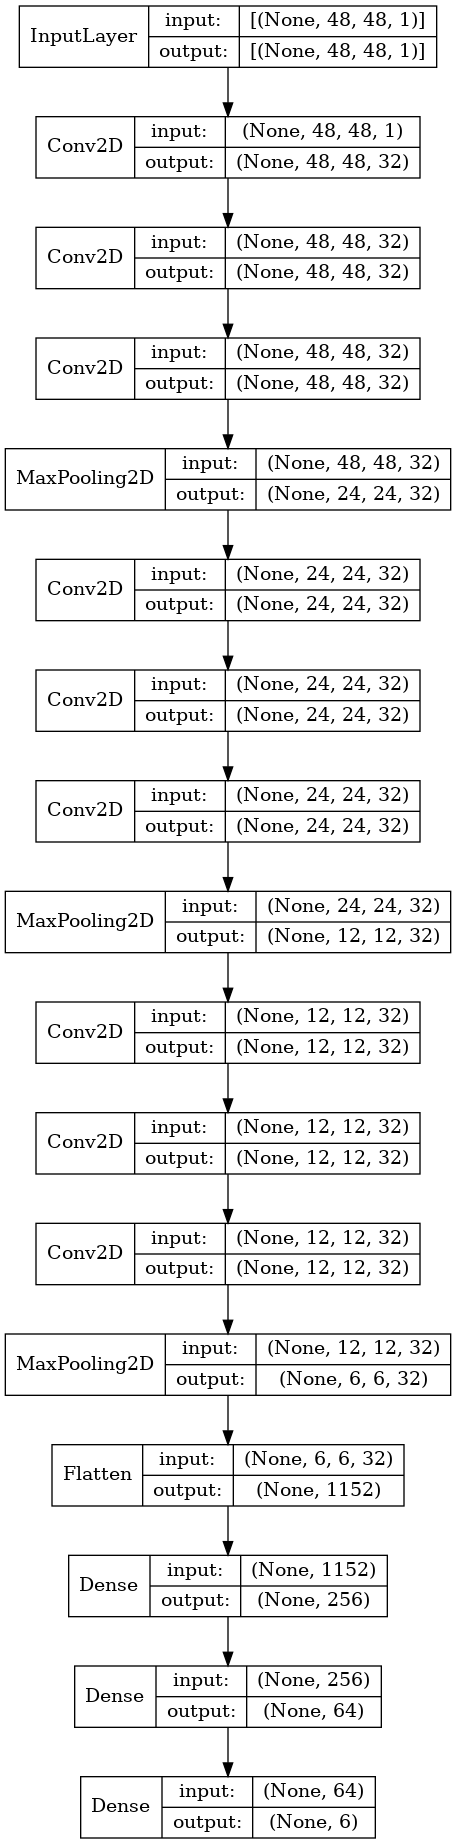
\includegraphics[scale=0.35]{Bilder/ModelSummary.png}
\caption{ Model Summary with several Layers and I/O Shapes }
\label{fig:Model Summary}
\end{figure}

\subsection{Trainieren des Modells}
Sobald das beschriebene Modell kreiert wurde, kann mit dem wesentlichen Teil, dem Trainieren, fortgefahren werden. Ein definiertes Modell besitzt in Keras die Funktion \texttt{fit} deren Verwendung im einfachsten Fall folgendermaßen aussieht: \texttt{fit(x=Trainingsdaten, y=Trainingslabels)}, wobei \texttt{x} und \texttt{y} in diesem Fall Numpy-Arrays sind. Die Trainingsdaten und die entsprechenden Labels erhalten wir aus dem Dataset, jedoch müssen diese noch in das erforderliche Format, eine Matrix bzw. ein Numpy-Array konvertiert werden. Dazu müssen die bereits erwähnten Zeichenketten von Pixeln in eine Matrix der Form 48 Pixel x 48 Pixel gebracht werden, wobei wiederum jedes Pixel als eindimensionales Array mit einem Element dargestellt wird. Sollten an dieser Stelle Farbbilder mit dem Format 48 Pixel x 48 Pixel als Input genutzt werden, hätte man anstatt der Struktur \texttt{(48, 48, 1)} Daten der Struktur \texttt{(48, 48, 3)} entsprechend der drei RGB-Werte. Optional können der Methode \texttt{fit} Validierungsdaten als Tupel mit zwei Numpy-Arrays, den Validierungsdaten und den zugehörigen Labels, übergeben werden. Diese müssen lediglich vorher analog zu den Trainingsdaten in ein passendes Format konvertiert werden.
Der Methode \texttt{fit} zum Trainieren des Modells können außerdem einige optionale Parameter mitgegeben werden, die im Zusammenhang mit den den Validierungsdaten besonders für die Optimierung des Modells, dem Hyperparameter-Tuning, wichtig sind.\newline
Als Rückgabewert liefert die angesprochene Methode ein History-Objekt, in welchem Daten wie Loss und Accuracy der Trainingsdaten und ggf. Loss und Accuracy der Validierungsdaten während des Trainingsprozesses aufgezeichnet wurden. Das History-Objekt existiert jedoch nur innerhalb der Laufzeit des Python-Skripts und wird nicht zusammen mit dem Modell über die API-Methode \texttt{save(path="modelToSave.model")} abgespeichert. Um sich die History eines Modells jederzeit anzeigen ausgeben und ggf. visualisieren zu können, werden die aufgezeichneten Daten zusätlich zum Modell im JSON-Format abespeichert und können bei Bedarf über entprechende Bibliotheken wieder geladen und in ein Dictionary konvertiert werden.\newline
Die Visualisierungen der aufgezeichneten Daten inklusive entsprechender Testdaten mithilfe der Bibliothek \texttt{matplotlib} können der Abbildung \ref{fig:Visualize History} entnommen werden.
\begin{figure}[h]
	\begin{minipage}[b]{\linewidth}
		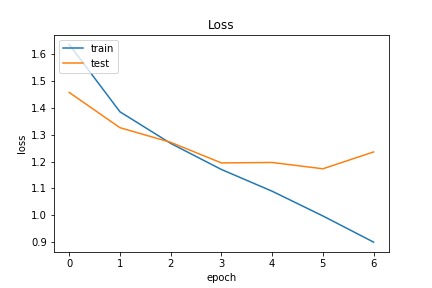
\includegraphics[width=\linewidth]{Bilder/loss_history.png}
	\end{minipage}
	\begin{minipage}[b]{\linewidth}
		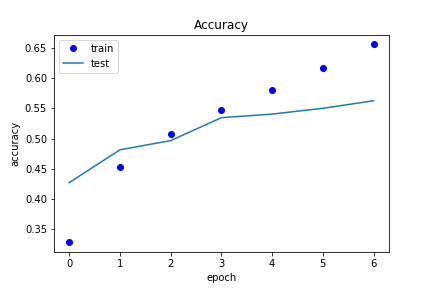
\includegraphics[width=\linewidth]{Bilder/accuracy_history.png}
	\end{minipage}
	\caption[t]{Visualisierung der aufgezeichneten Daten des History-Objektes}
	\label{fig:Visualize History}
\end{figure}

\subsection{Testen des Modells}
Beim Testen des Modells benötigt man analog zum Trainieren eines Modells mehrere Datensätze und deren jeweiligen Label. Anhand der Datensätze lässt man sich nun vom Trainierten Modell die Label vorhersagen und gleicht sie mit den tatsächlichen Labeln ab, um eine Genauigkeit zu ermitteln. Voraussetzung dafür ist, dass die Testdaten dem selben Format wie die Trainingsdaten, also einer \texttt{(48, 48, 1)}-Matrix, entsprechen. Mithilfe der Keras API-Methode \texttt{predict}, der man die gesamten Trainingsdaten auf einmal übergeben kann, kann man sich auf Grundlage des Modells die Label vorhersagen lassen. Die konkrete Rückgabe der Methode ist ein Array dessen Anzahl der Elemente der Anzahl an Trainingsdaten entspricht, wobei wiederum jedes Element selbst ein Array ist, dessen Länge der Anzahl an möglichen Emotionen entspricht. Übergibt man beispielsweise 10 Testdatensätze und das Modell wurde mit 4 Emotionen trainiert, erhält man ein zweidimensionales Array, welches 10 Arrays der Länge 4 enthält. In den inneren Feldern sind für jede Emotion Werte zwischen 0 und 1 enthalten, welche zusammen 1 ergeben. Vereinfacht gesagt wird für jede Emotion die als Input gegeben wird, die prozentuale Übereinstimmung mit jeder möglichen Emotion zurückgegeben bzw. die Wahrscheinlichkeit zu jeder möglichen Emotion vorhergesagt. Dies könnten beispielhaft so aussehen: \texttt{[0.05690899, 0.09713534, 0.5027235,  0.04000191, 0.29613075, 0.00709949]}. Möchte man zu einem Input eine einzige Emotion vorhersagen, ist es sinnvoll, die dem Maximum des Arrays entsprechende Emotion zurückzugeben. Nimmt man die in Tabelle \ref{tab:feremotions} definierte Zuordnung von Emotionen als Grundlage, entspricht das Maximum des Arrays dem Index 2, wobei dieser Wert wiederum der Emotion \texttt{Fear} zugeordnet ist.\newline
Gleicht man die vorhergesagten Emotionen mit den tatsächlichen Emotionen ab kann man eine statistische Auswertung über der Gesamtmenge aller Daten vornehmen, z.B. dass die Wahrscheinlichkeit einer richtigen Vorhersage bei 40\% liegt, oder den Anteil der richtigen Zuordnung jeder einzelnen Emotion, z.B. \texttt{[0.1, 0.2, 0.05, 0.15, 0.91, 0.34]}. Dem letzteren Beispiel kann man entnehmen, dass das Modell sehr gut geeignet ist, die Emotion die dem Wert 4 entspricht zu erkennen, jedoch sehr schlecht darin ist, alle anderen Emotionen zu erkennen. Beide Daten werden während des Testprozesses berechnet und sind bei der späteren Optimierung des Modells hilfreich.

\subsection{Optimierung des Modells}

\subsection{Webserver}
Einer der wesentlichen Unterschiede zu der zuvor entwickelten Lösung ist die Architektur. Es läuft nicht mehr alles lokal auf einem Rechner, sondern es zwischen Server und Client unterschieden. Alles was das Modell direkt betrifft, also das Trainieren, Testen und Vorhersagen geschieht auf dem Server, wo auch das Modell selbst existiert. 


Um mit dem Client interagieren zu können, wird das Webframework Flask verwendet, welches konkret als Webserver dient. Da Flask in Python geschrieben ist, wird die Implementierung von Endpunkten in Verbindung mit den bereits implementierten Funktionalitäten stark vereinfacht.\newline
Die Interaktion zwischen Server und Client ist sehr überschaubar und es wird lediglich ein einziger Endpunkt auf der Serverseite benötigt. Dieser Endpunkt nimmt mittels der \texttt{POST}-Methode ein vom Client geliefertes, grob vorbearbeitetes Bild entgegen. Dieses Bild wird dann auf dem Server so formatiert, dass mithilfe eines bereits trainierten Modells eine Emotionsvorhersage getroffen werden kann. Das Ergebnis wird dann an den Client zurückgeliefert und kann dort in einen entsprechenden Kontext wie die reine Ausgabe oder die Analyse eines Pokerfaces weiterverwendet werden.\newline
Damit der Server Vohersagen mithilfe eines Modells machen und Bilder archivieren kann, müssen zur Initialisierung das Modell geladen werden und entsprechende Ordnerstrukturen angelegt werden, sofern sie nicht vorhanden sind. Danach kann der Webserver gestartet werden, um Verbindungen vom Client über einen vordefinierten Port entgegenzunehmen. Sobald ein Client ein Bild ein den Server übergibt, wird dieses gespeichert bzw. archiviert. Da nicht sichergestellt ist, dass der Client ausschließlich Bilder auf denen nur ein Gesichtsausschnitt zu sehen ist und der Größe  48 Pixel x 48 Pixel entsprechen, muss dies zunächst serverseitig geprüft und ggf. angepasst werden.  
Die allgemeine Vorgehensweise ist dabei, zuerst ein Gesicht zu erkennen und dieses danach auf 48 Pixel x 48 Pixel zuzuschneiden. Damit das Modell eine optimale Vorhersage geben kann, muss der Ausschnitt des extrahierten Gesichtes ggf. noch in ein Graustufenformat konvertiert werden. Um nun einen validen Input für das Modell zu generieren, muss das Image-Objekt noch in einen Pixel-String bzw. in eine Matrixrepräsentation der Form \texttt{(48, 48, 1)} gebracht werden. Jetzt kann auf dem bei der Initialisierung geladenen Modell die bereits erläuterte Methode \texttt{predict} aufgerufen und die Vorhersagewerte an den Client zurückgegeben werden.

\subsection{Client}
Der Hauptzweck des Client-Anwendung ist die Darstellung des Output mithilfe einer grafischen Benutzerschnittstelle. Im Hintergrund interagiert der Client mit dem Server, indem er Webcam-Bilder liefert, die hinsichtlich der Emotion auf dem Server analysiert werden und erhält Vorhersage-Matrizen. Die Interpretation dieser Werte obliegt dem Client, der diese dem Nutzer auf bestimmte Weise zugänglich macht. Die Anwendung umfasst somit zwei Wesentliche Funktionalitäten, eine grafische Oberfläche zur Interaktion mit dem Anwender und im Hintergrund die Netzwerkkommunikation mit dem Server. Da nach den definierten Anforderungen keine komplexen Interaktionen mit dem Nutzer notwendig sind, umfasst die GUI lediglich ein Fenster in dem der Video-Stream der Webcam ausgegeben wird, mit der zusätlichen Information, ob sich laut Definition um ein Pokerface handelt oder nicht, als Schriftzug in einer Ecke des Bildes. Somit kann der Nutzer seine aktuelle Emotion sehen und die Ausgabe, ob ein Pokerface vorhanden ist oder nicht, besser nachvollziehen. Da die Ausgabe des Video-Streams im Fenster und die Netzwerkkommunikation grundsätzlich voneinander unabhängig sind, können diese Aufgaben in zwei verschiedene Prozesse bzw. Threads aufgeteilt werden. Wird dies nicht gemacht, kann es je nach Auslastung des Netzwerkes oder Ressourcenknappheit auf der Serverseite zu einer ruckeligen und verzögerten Ausgabe des Video-Stream kommen. Somit werden im Hauptprozess die grafischen Aufgaben erledigt, wobei man für die jeweilige Information, ob es sich um ein Pokerface handelt oder nicht, in eine geteilten globalen Variable gespeichert ist, die vom Netzwerk-Thread geschrieben und vom GUI-Thread gelesen wird. In definierten Intervallen kann der Thread zur Kommunikation mit dem Server einzelne Bilder des Video-Streams abgreifen und zur Vorhersage an den Server schicken, ohne dass bei der Ausgabe auf die Antwort des Servers gewartet werden muss. Wie bereits erwähnt, werden die vom Server gelieferten Daten clientseitig interpretiert, was konkret bedeutet, dass ein Algorithmus implementiert werden muss, der anhand der Vorhersagedaten entscheidet, ob ein Pokerface vorhanden ist oder nicht. \newline
Wie bereits beschrieben wertet der hier explizierte Algorithmus Eingabedaten aus einem Videostream aus um ein Pokerface festzustellen. Nach der Definition in Kaptiel 
\ref{pokerface}gibt es zwei Arten von Pokerfaces. Dieser Algorithmus behandelt dabei die Variante, in der das beobachtete Subjekt seinen Gesichtsausdruck dauerhaft beibehält. Um dies zu bewerkstelligen muss der Videostream in einer gewissen Rate abgetastet werden. Dies bedeutet, dass immer wieder Momentaufnahmen aus dem Videostream entnommen werden, und dem Server zum evaluieren gegeben werden. Dieser Vorgang wird einige Male wiederholt, und die daraus resultierenden Daten aggregiert und zwischengespeichert. Das Ergebnis dieser Aggregation ist dann eine Liste der Länge
$ n $  , wobei $ n \in N $	$ n $  , wobei $ n \in N $
Jedes Element dieser Liste ist wiederum eine Liste, die Emotionsvorhersagen für ein bestimmtes Bild aus dem Videostream beinhaltet. So könnte z.B. eine solche Liste der Länge 2 folgende Struktur aufweisen: \newline
$ \qquad[ [0.61, 0.30, 0.15, 0.01, 0.76, 0.95] , [0.31, 0.22, 0.51, 0.41, 0.01, 0.55] ] $
Wobei jeweils ein Wert für eine Emotion steht bzw. die Wahrscheinlichkeit einer Emotion für das jeweilige Bild. Anhand dieser Liste wird dann wiederum die Abweichung der Emotionen in den Bildern festgelegt. Dazu werden die einzelnen Emotionswerte zuerst extrahiert und zusammengefasst - also alle fröhlichen, ängstlichen, neutralen, etc. Danach werden dann die Unterschiede in den jeweiligen Werten ermittelt.
Dies geschieht, indem zuerst der Mittelwert einer Emotion ermittelt wird, und dann die Werte gegen diesen geprüft werden. Weicht dabei eine Emotionsvorhersage zu weit von dem Mittelwert ab, wird zurückgegeben, dass ein Pokerface nicht vorliegen kann, da der Gesichtsausdruck nicht beibehalten wurde. Ein Toleranzwerte muss wegen Messungenauigkeiten des Models eingeplant werden.
Formal beschrieben wertet der Algorithmus also folgende Formel aus: \newline
Sei $ Emotion $ eine Liste der Länge $ n $ mit den Daten einer Emotion aus der Eingabeliste, mit der Form $$ Emotion = \qquad [e_{1} \dots e_{n}] $$ 	
und $$avg =\frac{1}{n} \cdot \sum_{i = 0}^{n} e_{i} $$ so gilt:
\newline 
$$ \forall e_{i} \in Emotion : (avg - e_{i} ) \leq \epsilon \Rightarrow Pokerface = True $$	\newline
 $ \epsilon$ ist hierbei die Toleranz in der sich eine Abweichung der Emotion begeben darf.
\chapter{Ergebnis}
Außerdem werden die Aufgrund des erstellten Konzeptes entwickelten Lösungsansätze und Lösungen erläutert. Darin inbegriffen ist vor allem auch das trainierte Modell zum klassifizieren von den vordefinierten Emotionen und das Verifizieren und Testen dieses Modells.

\let\cleardoublepage\relax
\chapter{Diskussion}
Das nunmehr letzte Kapitel soll sich mit der kurzen Zusammenfassung der Ergebnisse des letztens Teils und deren Bewertung widmen. 
%Die Ergebnisse aus dem letzten Kapitel noch einmal zusammenfassen?
Des Weiteren sollen die angewandten Methoden reflektiert werden,
offene Fragen beantwortet und auch weitere Punkte aufgezeigt werden die verbessert oder noch implementiert werden können. Dazu soll zunächst die Ergebnisse kurz zusammengefasst werden.

\section{Reflexion der Ergebnisse}

\subsection{Alternativen}

\section{Reflexion Vorgehen}
Mehr darauf eingehen dass das Kontrovers ist und auch die Basisemotionen kontrovers sind --  aber keine andere Möglichkeit vorhanden 

\section{Reflexion der Literatur}
Bezüglich der Literatur ergeben sich nun einige Schwierigkeiten. Dies liegt unter anderem daran, dass das generelle Thema der Gesichts und Emotionserkennung immer noch vor allem aus
psychologischer Sicht in der Literatur behandelt wurde. Zwar gibt es Fachbücher auch aus informationstechnischer Sicht, welche ebenfalls in dieser Arbeit verwendet wurden.

\section{Offene Implikationen}

\chapter{Ausblick}

\section{Alternative Ansätze zur Umsetzung von Emotionserkennung}
In diesem Abschnitt nun werden verschiedene alternative Ansätze dargestellt und expliziert, die dazu verwendet werden können um Emotionen zu erkennen.
Dieses Unterkapitel beschäftigt sich mit alternativen Ansätzen zu den bereits explizierten Basisemotionen. Diese sind wie bereits erwähnt umstritten, was die Frage zulässt warum diese überhaupt
verwendet werden sollten. Ein weiterer kreativer Ansatz zur Erkennung von Emotionen wäre die Analyse der Stimmlage.
Dieser Ansatz beruft sich darauf, dass das Sprachzentrum eines Menschen einer der wichtigsten Aspekte der Kommunikation und somit auch der Preisgabe von Informationen über den emotionalen Zustand eines Individuums ist.
\footcite[Vgl. ][Abstract]{EmotionInSpeech}
Dieser Ansatz ist jedoch nicht zielführend, da hier hauptsächlich die Stimme analysiert wird. Von einer Stimme kann nun auf eine Emotion geschlossen werden. Für den Usecase ist dieser Ansatz allerdings ungeeignet, aus folgenden Gründen:\newline
Es kann möglich sein eine Emotion anhand der Sprache zu erkennen. Das Äquivalent eines Pokerfaces wäre dementsprechend eine neutrale Stimmlage, welche keine Emotionen suggeriert. Nun kann aber keine Aussage getroffen werden aus welchen Gründen eine Person neutral spricht. Es könnte von einem Pokerface stammen, oder einer monotonen Sprechweise, oder einen gelangweilten Gemütszustand. Dies ist nicht eindeutig identifizierbar. Gleiches könnte nicht über ein neutrales Gesicht gesagt werden, da dies gemeinhin als Pokerface bezeichnet wird. %Spricht das nicht auch gegen unser Vorgehen?
Ein weitere Ansatz wäre die Analyse der derzeit vernommenen Musik. Diese kann einem bestimmten Gemütszustand zugesprochen werden, welches auf eine aktuelle Emotion übertragbar ist.
\footcite[Vgl.][1]{MusicEmotion}
Ziel dieses Forschungszweiges ist es daher die hinter Liedern oder Klängen stehenden Emotionen zu ermitteln und diese entsprechend zu kategorisieren.
Dieser Ansatz erscheint zunächst durchaus interessant, hat jedoch genauso Nachteile wie die Analyse von Emotionen anhand von Bildern die Basisemotionen zeigen. %Spricht wieder gegen unser Vorgehen
Dieser liegt hier unter anderem in der Genauigkeit der Analysen. So z.B. lieferte ein Testprojekt an der Russischen HSE (Higher School of Economics) das Ergebnis von einer maximalen Genauigkeit von 71\%.
\footcite[Vgl. ][Abstract]{EmotionInSound}
In dem Versuchsaufbau wurden Spektrogramme von Klangfragmenten ausgewertet und versucht mittels Neuronalen Netzen eine Klassifikation der hinter dem Klang liegenden Emotion zu erreichen.
\footcite[Vgl. ][Abstract]{EmotionInSound}
Der generelle Ansatz anhand von Musik die Emotion eines Individuums abzulesen ist zwar praktikabel und von dem Versuchsaufbau auch vergleichbar zu dem Ansatz bereits gelabelte Bilder zu verwenden. Jedoch lässt sich auf diese Weise aus zwei Gründen nicht die eigentliche Zielaufgabenstellung ableiten, das Erkennen eines Pokerfaces. Zum einen handelt es sich in dieser Arbeit um eine visuelle Problemstellung, in welcher das Erkennen des Gemütszustandes anhand des Gesichtsausdruckes erkannt werden soll, also einem vorhandenen bzw. nicht vorhandenen Pokerface. Zum anderen würde die Analyse von Musik einen Rückschluss auf den allgemeinen Gemütszustand des Betroffenen folgern und nicht eine kurzzeitige Stimmungsschwankung aufgrund beispielsweise eines schlechten Blattes, wie in diesem Usecase.

\let\cleardoublepage\relax
\newpage

\printbibheading
\printbibliography[type=book,heading=subbibliography,title={Literaturquellen}]
\pagestyle{empty}
\printbibliography[type=misc,heading=subbibliography,title={Sonstige Quellen}]
\pagestyle{empty}
\newpage
\pagestyle{empty}

\end{document}
